%杨舒云的实验报告编辑界面,使用了Huanyu Shi,2019级的模板,杨舒云在此拜谢ORZ!

%!TEX program = xelatex
\documentclass[dvipsnames, svgnames,a4paper,11pt]{article}
% ----------------------------------------------------- 
%	加边框的命令
%	参考:https://tex.stackexchange.com/questions/531559/how-to-add-the-page-border-for-first-two-pages-in-latex
\usepackage{tikz}
\usetikzlibrary{calc}
\usepackage{eso-pic}
\AddToShipoutPictureBG{%
\begin{tikzpicture}[overlay,remember picture]
\draw[line width=0.6pt] % 边框粗细
    ($ (current page.north west) + (0.6cm,-0.6cm) $)
    rectangle
    ($ (current page.south east) + (-0.6cm,0.6cm) $); % 边框位置
\end{tikzpicture}}


\usepackage{xcolor}
\definecolor{c1}{HTML}{086173} % 目录颜色 原版为2752C9 紫灰色535AAA 蓝紫色0B0DB7 深蓝色070F94 湖绿色219394 松石灰绿086173
\definecolor{c2}{HTML}{E20129} % 引用颜色 原版\definecolor{c2}{RGB}{190,20,83} 橙色F24729

\usepackage{ctex}
\usepackage[top=28mm,bottom=28mm,left=15mm,right=15mm]{geometry}
\usepackage{hyperref} 
\hypersetup{
	colorlinks,
	linktoc = section, % 超链接位置,选项有section, page, all
	linkcolor = c1, % linkcolor 目录颜色
	citecolor = c1  % citecolor 引用颜色
}
\usepackage{amsmath,enumerate,multirow,float}
\usepackage{tabularx}
\usepackage{tabu}
\usepackage{subfig}
\usepackage{fancyhdr}
\usepackage{graphicx}
\usepackage{wrapfig}  
\usepackage{physics}
\usepackage{appendix}
\usepackage{amsfonts}

%
\usepackage{tcolorbox}
\tcbuselibrary{skins,breakable}
\newtcolorbox{tbox}[2][]{
    colframe=black!70!,
    breakable,
    enhanced,
	boxrule =0.5pt,
    title = {#2},
    fonttitle = \large\kaishu\bfseries,
	drop fuzzy shadow,
    #1
}
\newtcolorbox[auto counter,number within=section]{question}[1][]{
  top=2pt,bottom=2pt,arc=1mm,
  boxrule=0.5pt,
%   frame hidden,
  breakable,
  enhanced, %跨页后不会显示下边框
  coltitle=c1!80!gray,
  colframe=c1,
  colback=c1!3!white,
  drop fuzzy shadow,
  title={思考题~\thetcbcounter:\quad},
  fonttitle=\bfseries,
  attach title to upper,
  #1
}

% ---------------------------------------------------------------------
%	利用cleveref改变引用格式,\cref是引用命令
\usepackage{cleveref}
\crefformat{figure}{#2{\textcolor{c2}{Figure #1}}#3} % 图片的引用格式
\crefformat{equation}{#2{(\textcolor{c2}{#1})}#3} % 公式的引用格式
\crefformat{table}{#2{\textcolor{c2}{Table #1}}#3} % 表格的引用格式


% ---------------------------------------------------------------------
%	页眉页脚设置
\fancypagestyle{plain}{\pagestyle{fancy}}
\pagestyle{fancy}
\lhead{\kaishu 中山大学物理与天文学院电子技术实验\uppercase\expandafter{\romannumeral1}} % 左边页眉,学院 + 课程
\rhead{\kaishu 实验报告By杨舒云\&戴鹏辉} % 右边页眉,实验报告标题
\cfoot{\thepage} % 页脚,中间添加页码


% ---------------------------------------------------------------------
%	对目录、章节标题的设置
\renewcommand{\contentsname}{\centerline{\huge 目录}}
\usepackage{titlesec}
\usepackage{titletoc}
% \titleformat{章节}[形状]{格式}{标题序号}{序号与标题间距}{标题前命令}[标题后命令]
\titleformat{\section}{\centering\LARGE\songti}{}{1em}{}

% ---------------------------------------------------------------------
%   listing代码环境设置
\usepackage{listings}
\lstloadlanguages{python}
\lstdefinestyle{pythonstyle}{
backgroundcolor=\color{gray!5},
language=python,
frameround=tftt,
frame=shadowbox, 
keepspaces=true,
breaklines,
columns=spaceflexible,                   
basicstyle=\ttfamily\small, % 基本文本设置,字体为teletype,大小为scriptsize
keywordstyle=[1]\color{c1}\bfseries, 
keywordstyle=[2]\color{Red!70!black},   
stringstyle=\color{Purple},       
showstringspaces=false,
commentstyle=\ttfamily\scriptsize\color{green!40!black},%注释文本设置,字体为sf,大小为smaller
tabsize=2,
morekeywords={as},
morekeywords=[2]{np, plt, sp},
numbers=left, % 代码行数
numberstyle=\it\tiny\color{gray}, % 代码行数的数字字体设置
stepnumber=1,
rulesepcolor=\color{gray!30!white}
}




% ---------------------------------------------------------------------
%	其他设置
\def\degree{${}^{\circ}$} % 角度
\graphicspath{{./images/}} % 插入图片的相对路径
\allowdisplaybreaks[4]  %允许公式跨页 
\usepackage{lipsum}
\usepackage{adjustbox}
\usepackage{tabularray}
%\usepackage{mathrsfs} % 字体
\captionsetup[figure]{name=Figure} % 图片形式
\captionsetup[table]{name=Table} % 表格形式

\begin{document}
	
	
	
	% 实验报告封面	
	
	% 顶栏
	\begin{table}
		\renewcommand\arraystretch{1.7}
		\begin{tabularx}{\textwidth}{
				|X|X|X|X
				|X|X|X|X|}
			\hline
			\multicolumn{2}{|c|}{预习报告}&\multicolumn{2}{|c|}{实验记录}&\multicolumn{2}{|c|}{分析讨论}&\multicolumn{2}{|c|}{总成绩}\\
			\hline
			\LARGE25 & & \LARGE25 & & \LARGE30 & & \LARGE80 & \\
			\hline
		\end{tabularx}
	\end{table}
	% ---
	
	% 信息栏
	\begin{table}
		\renewcommand\arraystretch{1.7}
		\begin{tabularx}{\textwidth}{|X|X|X|X|}
			\hline
			年级、专业: & 2022级 物理学 &组号: & E2\\
			\hline
			姓名: & 戴鹏辉、杨舒云  & 学号: & 22344016、22344020\\
			\hline
			实验时间: & 2024/4/10 & 教师签名: & \\
			\hline
		\end{tabularx}
	\end{table}
	% ---
	
	% 大标题
	\begin{center}
		\LARGE ET1-6 \quad R、L、C元件阻抗特性研究
	\end{center}
	% ---
	
	% 注意事项
	
	% 基本
	\textbf{【实验报告注意事项】}
	\begin{enumerate}
		\item 实验报告由三部分组成:
		\begin{enumerate}
			\item 预习报告:课前认真研读实验讲义,弄清实验原理;实验所需的仪器设备、用具及其使用、完成课前预习思考题;了解实验需要测量的物理量,并根据要求提前准备实验记录表格(可以参考实验报告模板,可以打印)。\textcolor{red}{\textbf{(20分)}}
			\item 实验记录:认真、客观记录实验条件、实验过程中的现象以及数据。实验记录请用珠笔或者钢笔书写并签名(\textcolor{red}{\textbf{用铅笔记录的被认为无效}})。\textcolor{red}{\textbf{保持原始记录,包括写错删除部分,如因误记需要修改记录,必须按规范修改。}}(不得输入电脑打印,但可扫描手记后打印扫描件);离开前请实验教师检查记录并签名。\textcolor{red}{\textbf{(30分)}}
			\item 数据处理及分析讨论:处理实验原始数据(学习仪器使用类型的实验除外),对数据的可靠性和合理性进行分析;按规范呈现数据和结果(图、表),包括数据、图表按顺序编号及其引用;分析物理现象(含回答实验思考题,写出问题思考过程,必要时按规范引用数据);最后得出结论。\textcolor{red}{\textbf{(30分)}}
		\end{enumerate}
		\textbf{实验报告就是将预习报告、实验记录、和数据处理与分析合起来,加上本页封面。\textcolor{red}{(80分)}}
		\item 每次完成实验后的一周内交\textbf{实验报告}(特殊情况不能超过两周)。
		\item \textbf{其它注意事项}:
		\begin{enumerate}
			\item 请认真查看并理解实验讲义第一章内容;
			\item 注意实验器材的合理使用;
			\item 使用结束使用各种仪器之后需要将其放回原位。
		\end{enumerate}
	\end{enumerate}
	
	% 安全
	\textbf{【实验安全注意事项】}	
	\begin{enumerate}
		\item 采用万用表交流电压档测量交流电压时,请注意有效频率范围。
		\item 在使用示波器测量电压或相位差时,注意示波器两个通道输入信号的接地点接法必须保证信号源、示波器所有通道的接地点接在电路的同一个点上。
		\item 在使用示波器测量电压或相位差时,示波器输入信号的耦合方式要选择交流耦合。
		\item 绘制幅频特性和相频特性曲线时,频率轴采用对数坐标。
		\item 在计算时请注意角频率与频率的转换。
		
	\end{enumerate}
	
	% ---
	
	% 特别鸣谢
	\textbf{【特别鸣谢及模板说明】}	
	
	感谢2019级学长石寰宇为本实验报告提供\LaTeX 模板。\textcolor{red}{\textbf{由于原实验报告模板缺少实验编号,为方便在电脑上整理,故添加自命名编号ET1-6}}
	% ---
	
	
	
	% 目录
	\clearpage
	\tableofcontents
	\clearpage
	% ---
	
	
	
	% 预习报告	
	
	% 小标题
	\setcounter{section}{0}
	\section{ET1-6 \quad R、L、C元件阻抗特性研究 \quad\heiti 预习报告}
	% ---
	
	% 实验目的
	\subsection{实验目的}
	\begin{enumerate}
		\item 测量电阻、感抗、容抗与频率的关系,测定$R$-$f$、$X_L$-$f$及$X_c$-$f$特性曲线。
		\item 观察并了解$R$、$L$、$C$元件两端电压与电流间的相位关系。
		
	\end{enumerate}
	% ---
	
	% 仪器用具
	\subsection{仪器用具}
	\begin{table}[htbp]
		\centering
		\renewcommand\arraystretch{1.6}
		% \setlength{\tabcolsep}{10mm}
		\begin{tabular}{p{0.05\textwidth}|p{0.20\textwidth}|p{0.05\textwidth}|p{0.5\textwidth}}
			\hline
			编号& 仪器用具名称 & 数量 &  主要参数(型号,测量范围,测量精度等) \\
			\hline
			1&  电路原理箱或板& 1 &  \\
			\hline
			2&  函数信号发生器& 1 &  \\
			\hline
			3&  交流毫伏表& 1 &  \\
			\hline
			4&  直流电压表或万用表& 1 & 0~30V \\
			\hline
			5&  2号实验导线& N & 二端2号镀金插头 \\
			\hline
		\end{tabular}
	\end{table}
	% ---
	
	% 原理概述
	\subsection{原理概述}
	\begin{enumerate}
		\item 阻抗频率特性
		
		在正弦交流信号作用下,$R$、$L$、$C$电路元件在电路中的抗流作用与信号的频率有关,它们的阻抗频率特性$R$-$f$、$X_L$-$f$及$X_c$-$f$曲线如\cref{fig:graph1-1}所示。
		
		\begin{figure}[htbp]
			\centering
			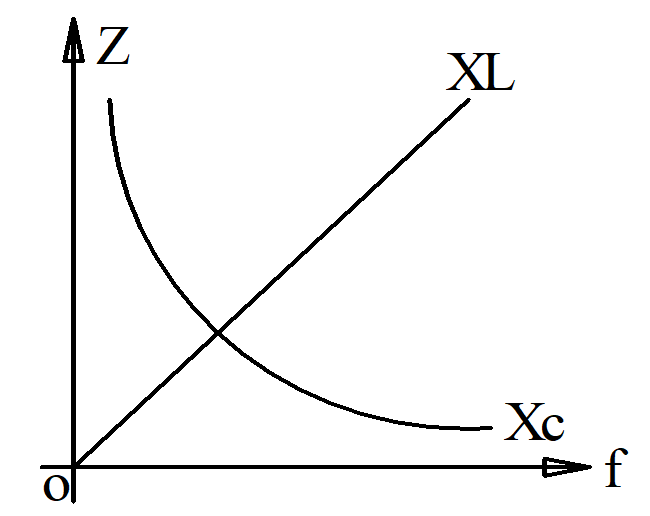
\includegraphics[width=0.4\textwidth]{graph1-1.png}
			\caption{$R$、$L$、$C$电路元件阻抗频率特性}
			\label{fig:graph1-1}
		\end{figure}
		
		\item 阻抗三角形
		
		\begin{figure}[htbp]
			\centering
			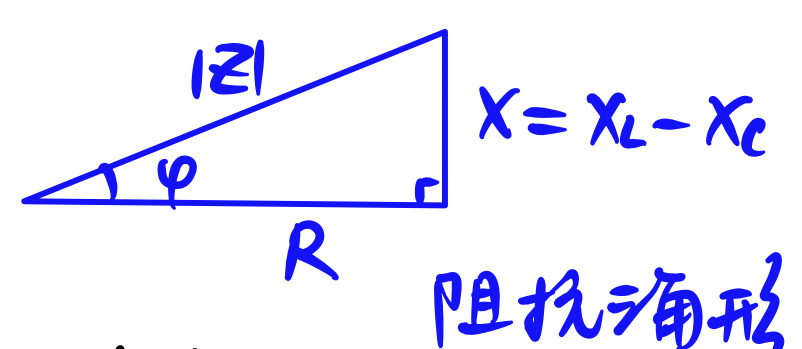
\includegraphics[width=0.5\textwidth]{ET1_6GraB1.png}
			\caption{阻抗三角形}
			\label{fig:figB1}
		\end{figure}
		
		电阻 (R):电阻的阻抗是纯实数,不随频率变化。电阻的阻抗表达式为 \( Z_R = R \),其中 \( R \) 是电阻的阻值。
		
		电感 (L):电感的阻抗包含实部和虚部,主要特性是其阻抗随频率增加而增加。电感的阻抗表达式为 \( Z_L = j\omega L \),其中 \( \omega \) 是角频率,\( L \) 是电感值,\( j \) 是虚数单位。
		
		电容 (C):电容的阻抗同样包含实部和虚部,但其主要特性是阻抗随频率增加而减小。电容的阻抗表达式为 \( Z_C = \frac{1}{j\omega C} \),其中 \( C \) 是电容值。
		
		阻抗三角形:
		对于电感,阻抗向量在复平面的正虚轴方向。
		对于电容,阻抗向量在复平面的负虚轴方向。
		对于电阻,阻抗向量在实轴上。
		
		这样,如果你画一个复平面图,电阻阻抗向量会沿实轴延伸,电感的阻抗向量会垂直向上延伸,而电容的阻抗向量则垂直向下延伸。这三种元件的组合可以形成一个阻抗三角形,其中垂直边代表电感和电容的反应性部分(虚部),水平边代表电阻的阻抗部分(实部)。
		
		\item 幅频特性曲线
		
		\begin{figure}[htbp]
			\centering
			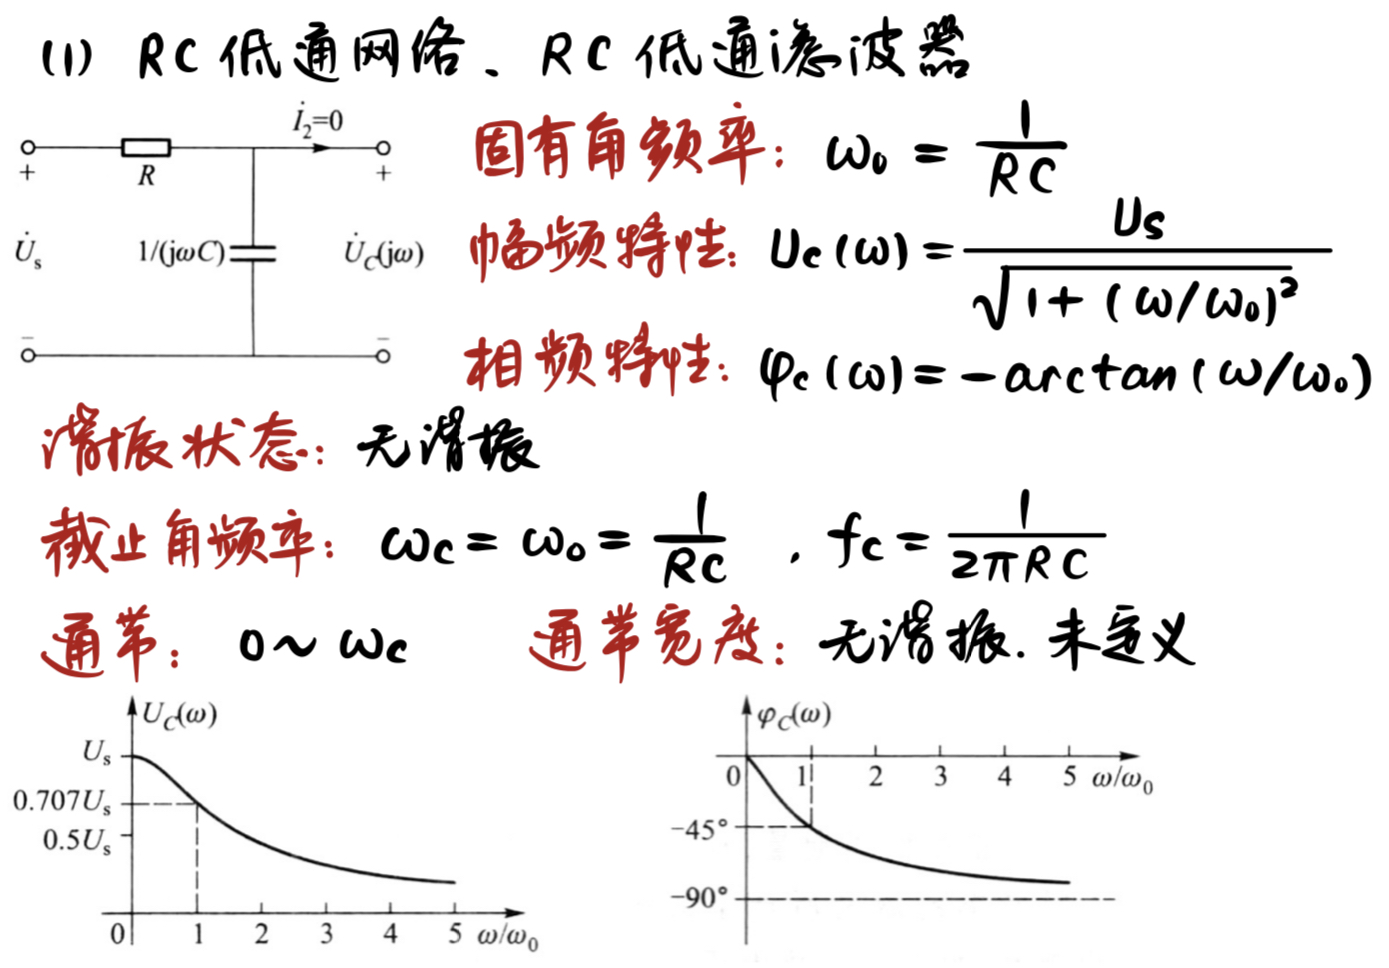
\includegraphics[width=0.5\textwidth]{ET1_6GraB2.png}
			\caption{幅频特性曲线与相频特性曲线}
			\label{fig:figB2}
		\end{figure}
		
		\begin{figure}[htbp]
			\centering
			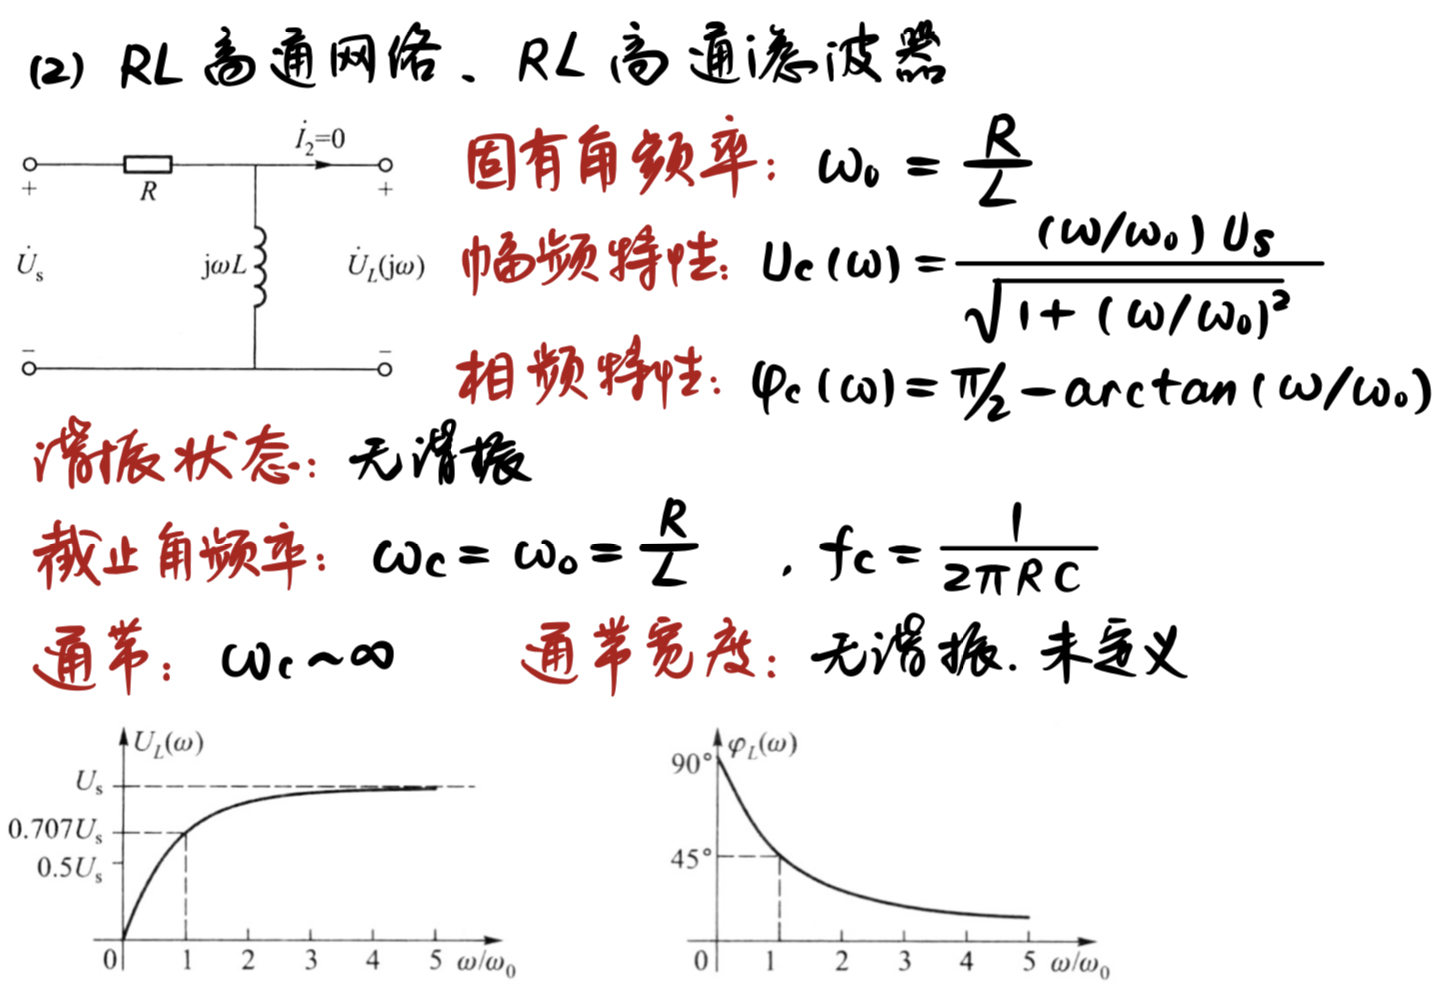
\includegraphics[width=0.5\textwidth]{ET1_6GraB3.png}
			\caption{幅频特性曲线与相频特性曲线}
			\label{fig:figB3}
		\end{figure}
		
		幅频特性曲线描述了电路元件对不同频率信号的响应程度,这是分析电阻、电感和电容在交流电路中行为的重要工具。下面详细介绍每种元件的幅频特性曲线:
		
		电阻 (R):
		电阻的幅频特性是平坦的,意味着电阻的阻抗不随频率变化。电阻的阻抗为 \(Z_R = R\),是一个实数,与频率无关。因此,无论信号的频率如何,电阻的幅值都保持恒定。
		
		电感 (L):
		电感的幅频特性曲线随频率增加而上升。电感的阻抗为 \(Z_L = j\omega L\),其中 \(j\) 是虚数单位,\(\omega = 2\pi f\) 是角频率,\(f\) 是信号频率,\(L\) 是电感值。因此,电感的阻抗幅值 \(|Z_L| = \omega L\) 随频率增加而线性增加。这表示电感对高频信号的阻抗较大,而对低频信号的阻抗较小。
		
		电容 (C):
		电容的幅频特性曲线随频率增加而下降。电容的阻抗为 \(Z_C = \frac{1}{j\omega C}\),因此电容的阻抗幅值 \(|Z_C| = \frac{1}{\omega C}\) 随频率增加而减少。这意味着电容对低频信号的阻抗较大,而对高频信号的阻抗较小,电容在高频下几乎不阻碍电流的流动。
		
		这三种元件的幅频特性对于设计滤波器、调谐电路和各种频率选择电路非常重要。电阻在所有频率下提供稳定的阻抗,而电感和电容则允许电路在不同频率下表现出不同的行为,这可以用来阻挡或通过特定频率范围的信号。
		
		\item 相频特性曲线
		
		相频特性曲线描述了电路元件的相位响应随频率的变化,这对于理解交流电路中信号的相位变化至关重要。下面详细介绍电阻、电感和电容的相频特性曲线:
		
		电阻 (R):
		电阻的相频特性是常数,因为电阻的阻抗没有虚部,所以其相位角始终为0度。这意味着通过电阻的电压和电流在所有频率下都是同相的。在相频特性曲线上,电阻的线是水平的,表示在任何频率下相位都不改变。
		
		电感 (L):
		电感的阻抗为 \(Z_L = j\omega L\),其相位角为+90度,因为阻抗的虚部为正,实部为0。这表示电感使得通过它的电流相对于电压滞后90度。在电感的相频特性曲线上,无论频率如何变化,相位角始终是+90度,所以这条线也是水平的。
		
		电容 (C):
		电容的阻抗为 \(Z_C = \frac{1}{j\omega C}\),其相位角为-90度,因为阻抗的虚部为负,实部为0。这表示电容使得通过它的电流相对于电压超前90度。在电容的相频特性曲线上,无论频率如何变化,相位角始终是-90度,因此这条线也是水平的。
		
		总结来说,电阻、电感和电容的相频特性曲线都是水平线,但是它们的相位值不同。电阻的相位角为0度,电感的相位角为+90度,电容的相位角为-90度。这些特性对于设计需要精确相位控制的电路非常重要,例如在信号处理和通信系统中。	

	\end{enumerate}
	% ---
	
	
	
	% 实验前思考题
	\subsection{实验预习题}
	

		% 思考题1
		\begin{question}
			正弦稳态电路中采用向量法简化计算。
		\end{question}
		在正弦稳态电路中,采用向量法(也称为相量法或复数法)可以显著简化电路分析,尤其是在处理交流电路的相位和幅度问题时。这种方法依赖于将正弦波形的电压和电流表示为旋转的向量或复数。以下是如何使用向量法简化正弦稳态电路计算的步骤:
		
		1. 表示为相量
		将所有交流电压和电流表示为复数形式的相量。对于幅度为 \( V \)、频率为 \( f \)、初相位为 \( \phi \) 的电压,可以表示为:
		\[ \hat{V} = V \angle \phi \]
		这里 \( V \) 是幅值,\( \phi \) 是相位角(度或弧度),相量表示复数形式,利用 Euler 公式 \( e^{j\phi} = \cos \phi + j \sin \phi \) 转换为:
		\[ \hat{V} = V (\cos \phi + j \sin \phi) \]
		
		2. 使用复阻抗
		为电路中的每个元件指定相应的复阻抗:
		电阻 \( R \) 的阻抗为 \( Z_R = R \)
		电感 \( L \) 的阻抗为 \( Z_L = j\omega L \)
		电容 \( C \) 的阻抗为 \( Z_C = \frac{1}{j\omega C} \)
		这里 \( \omega = 2\pi f \) 是角频率。
		
		3. 应用基本电路定律
		使用基尔霍夫电压定律(KVL)和基尔霍夫电流定律(KCL)以及欧姆定律,但应用于复数形式的相量和阻抗。
		
		4. 解复数方程
		求解由第3步建立的复数方程组。这可以通过代数运算简化,例如复数加法、乘法和除法。
		
		5. 解析结果
		将复数形式的结果解析为实际物理量。计算每个相量的幅度和相位,转换回时域表达式。例如,如果电压相量为 \( \hat{V} = V (\cos \phi + j \sin \phi) \),则实际电压波形为:
		\[ v(t) = V \cos(2\pi ft + \phi) \]

		% 思考题2
		\begin{question}
			时域和频域表达方式的互相转换。
		\end{question}
		在信号处理和系统分析中,时域和频域之间的转换是一个非常重要的主题。理解这两种表达方式如何互相转换对于深入分析信号和系统的行为至关重要。这里我们详绀讨论两种主要的转换方法:傅里叶变换和逆傅里叶变换。
		
		1. 傅里叶变换(从时域到频域)
		
		傅里叶变换是一种将时域信号转换为频域信号的数学工具。它将时间函数(时域)分解为不同频率的正弦波和余弦波的组合(频域)。对于连续信号 \(x(t)\),其傅里叶变换定义为:
		\[ X(f) = \int_{-\infty}^\infty x(t) e^{-j 2\pi ft} \, dt \]
		这里 \(X(f)\) 是复数函数,表示频域中的振幅和相位,\(f\) 是频率。
		
		振幅谱:\( |X(f)| \) 描述了各个频率成分的振幅。
		相位谱:\( \arg(X(f)) \) 描述了各个频率成分的相位。
		
		2. 逆傅里叶变换(从频域到时域)
		
		逆傅里叶变换用于将频域信号转换回时域信号。如果已知频域表示 \(X(f)\),其逆变换定义为:
		\[ x(t) = \int_{-\infty}^\infty X(f) e^{j 2\pi ft} \, df \]
		这样,我们可以从频域数据恢复原始的时域信号。
		
		讨论应用
		
		信号分析:通过傅里叶变换,可以分析信号包含哪些频率成分,这对于诸如语音处理、音频编码等应用至关重要。
		系统特性:系统对不同频率的响应可以通过频域分析获得。例如,在电子和通信领域,通过系统的频率响应可以理解其滤波和放大特性。
		去噪和滤波:在频域中,可以更容易地识别并滤除噪声成分,这在图像处理和信号恢复中特别有用。
		压缩:频域分析还可以用于数据压缩,通过消除人类感知不到的频率成分,来减少数据的大小。
		
		% 思考题3
		\begin{question}
			阻抗三角形、电压向量三角形和功率三角形。
		\end{question}
		阻抗三角形、电压向量三角形和功率三角形是电力工程和电路分析中常用的几何工具,用于描述和分析电路的电气特性。这些三角形有助于直观地理解电路的行为和相互关系。下面将详细介绍每一个。
		
		1. 阻抗三角形
		阻抗三角形是用来表示电阻、电感和电容在交流电路中的总阻抗(复阻抗)的关系。阻抗 \( Z \) 可以表示为:
		\[ Z = R + jX \]
		其中,\( R \) 是电阻部分(实部),\( X \) 是电抗部分(虚部),包括电感性电抗 \( X_L \) 和容性电抗 \( X_C \)。
		
		电抗:
		电感性电抗 \( X_L = \omega L \),向上延伸。
		容性电抗 \( X_C = -\frac{1}{\omega C} \),向下延伸。
		
		在阻抗三角形中:
		水平轴(实轴)表示电阻 \( R \)。
		垂直轴(虚轴)表示总电抗 \( X = X_L + X_C \)。
		斜边表示总阻抗 \( |Z| = \sqrt{R^2 + X^2} \)。
		角度 \( \theta \) 表示阻抗的相位角,\( \tan(\theta) = \frac{X}{R} \)。
		
		2. 电压向量三角形
		电压向量三角形用于表示在具有电阻和电抗的电路中电源电压与电路各部分电压之间的关系。如果电路中有电阻 \( R \) 和电抗 \( X \),则总电压 \( V \) 可以分解为:
		\( V_R = IR \) 沿实轴(与电流 \( I \) 同相)。
		\( V_X = IX \) 沿虚轴(与电流 \( I \) 正交)。
		
		在电压向量三角形中:
		水平轴表示 \( V_R \)。
		垂直轴表示 \( V_X \)。
		斜边表示总电压 \( V = \sqrt{V_R^2 + V_X^2} \)。
		角度 \( \theta \) 与阻抗三角形的相位角相同。
		
		3. 功率三角形
		功率三角形用于描述功率的三个组成部分:实功 \( P \)、无功 \( Q \) 和视在功率 \( S \)。它们定义为:
		实功 \( P = VI \cos(\theta) \):电路中实际做功的部分,单位为瓦特 (W)。
		无功 \( Q = VI \sin(\theta) \):电路中储存并周期性交换的能量,单位为乏特 (VAR)。
		视在功率 \( S = VI \):电路总的电力需求,单位为伏安 (VA)。
		
		在功率三角形中:
		水平轴表示实功 \( P \)。
		垂直轴表示无功 \( Q \)。
		斜边表示视在功率 \( S \)。
		角度 \( \theta \) 是电压和电流之间的相位差。
		
		% 思考题4
		\begin{question}
			RC和RL电路的频率特性分析。
		\end{question}
		RC(电阻-电容)和RL(电阻-电感)电路的频率特性对于理解各种电子和通信系统中的信号处理至关重要。这些频率特性决定了电路如何响应不同频率的输入信号。我们将分别分析这两种电路的幅频和相频特性。
		
		1. RC 电路
		RC 电路通常用作低通或高通滤波器,具体取决于电阻和电容的连接方式。
		
		低通 RC 电路
		配置:电阻与电容串联,输出电压在电容两端取出。
		传递函数:
		\[
		H(f) = \frac{1}{1 + j \omega RC}
		\]
		其中,\(\omega = 2\pi f\) 是角频率,\(R\) 和 \(C\) 分别是电阻和电容的值。
		
		幅频特性:
		随着频率增加,输出信号的幅度减小。截止频率 \(f_c\) 由下式给出:
		\[
		f_c = \frac{1}{2\pi RC}
		\]
		在 \(f_c\),输出信号的幅度是最大幅度的 \(1/\sqrt{2}\)。
		
		相频特性:
		相位滞后从 0 度(在低频时)渐变到 -90 度(在高频时)。相位角为:
		\[
		\theta = -\arctan(\omega RC)
		\]
		
		高通 RC 电路
		配置:电阻与电容串联,输出电压在电阻两端取出。
		传递函数:
		\[
		H(f) = \frac{j \omega RC}{1 + j \omega RC}
		\]
		
		幅频特性:
		随着频率的增加,输出信号的幅度增加。截止频率与低通滤波器相同。
		
		相频特性:
		相位从 -90 度(在低频时)渐变到 0 度(在高频时)。
		
		2. RL 电路
		RL 电路常用作高通滤波器,根据输出是在电阻还是电感上取,其特性有所不同。
		
		RL 电路(电感在前,电阻在后)
		配置:电感与电阻串联,输出电压在电阻两端取出。
		传递函数:
		\[
		H(f) = \frac{R}{R + j \omega L}
		\]
		
		幅频特性:
		随着频率的增加,输出信号的幅度逐渐趋近于最大值。截止频率由下式给出:
		\[
		f_c = \frac{R}{2\pi L}
		\]
		在 \(f_c\),幅度达到最大幅度的 \(1/\sqrt{2}\)。
		
		相频特性:
		相位从 0 度(在低频时)渐变到 -90 度(在高频时)。

	% ---
	
	
	
	% 实验记录	
	\clearpage
	
	% 顶栏
	\begin{table}
		\renewcommand\arraystretch{1.7}
		\centering
		\begin{tabularx}{\textwidth}{|X|X|X|X|}
			\hline
			专业: & 物理学 & 年级: & 2022级 \\
			\hline
			姓名: & 戴鹏辉、杨舒云 & 学号: & 22344016、22344020\\
			\hline
			室温: & 26\degree C & 实验地点: & A522 \\
			\hline
			学生签名:& 见\textbf{附件}部分 & 评分: &\\
			\hline
			实验时间:& 2024/4/10 & 教师签名:&\\
			\hline
		\end{tabularx}
	\end{table}
	% ---
	
	% 小标题
	\section{ET1-6 \quad R、L、C元件阻抗特性研究  \quad\heiti 实验记录}
	% ---
	
	% 实验过程记录
	\subsection{实验内容、步骤与结果}
	
	%
	\subsubsection{操作步骤记录}
	\begin{enumerate}
		\item 测量R、L、C元件的阻抗频率特性
		
		通过函数信号发生器输出正弦信号接至如图2电路,作为激励源$u_s$,并用台式万用表交流电压档或示波器测量,激励电压设置为正弦信号输出,无直流偏置,有效值$U_{RMS}$=3V,并在实验过程中保持不变(比较麻烦);也可以固定设置函数信号发生器的电压输出值,引入函数发生器的内阻进行理论计算。

			\begin{figure}[htbp]
				\centering
				\subfloat[RC电路的阻抗频率特性电路图]
				{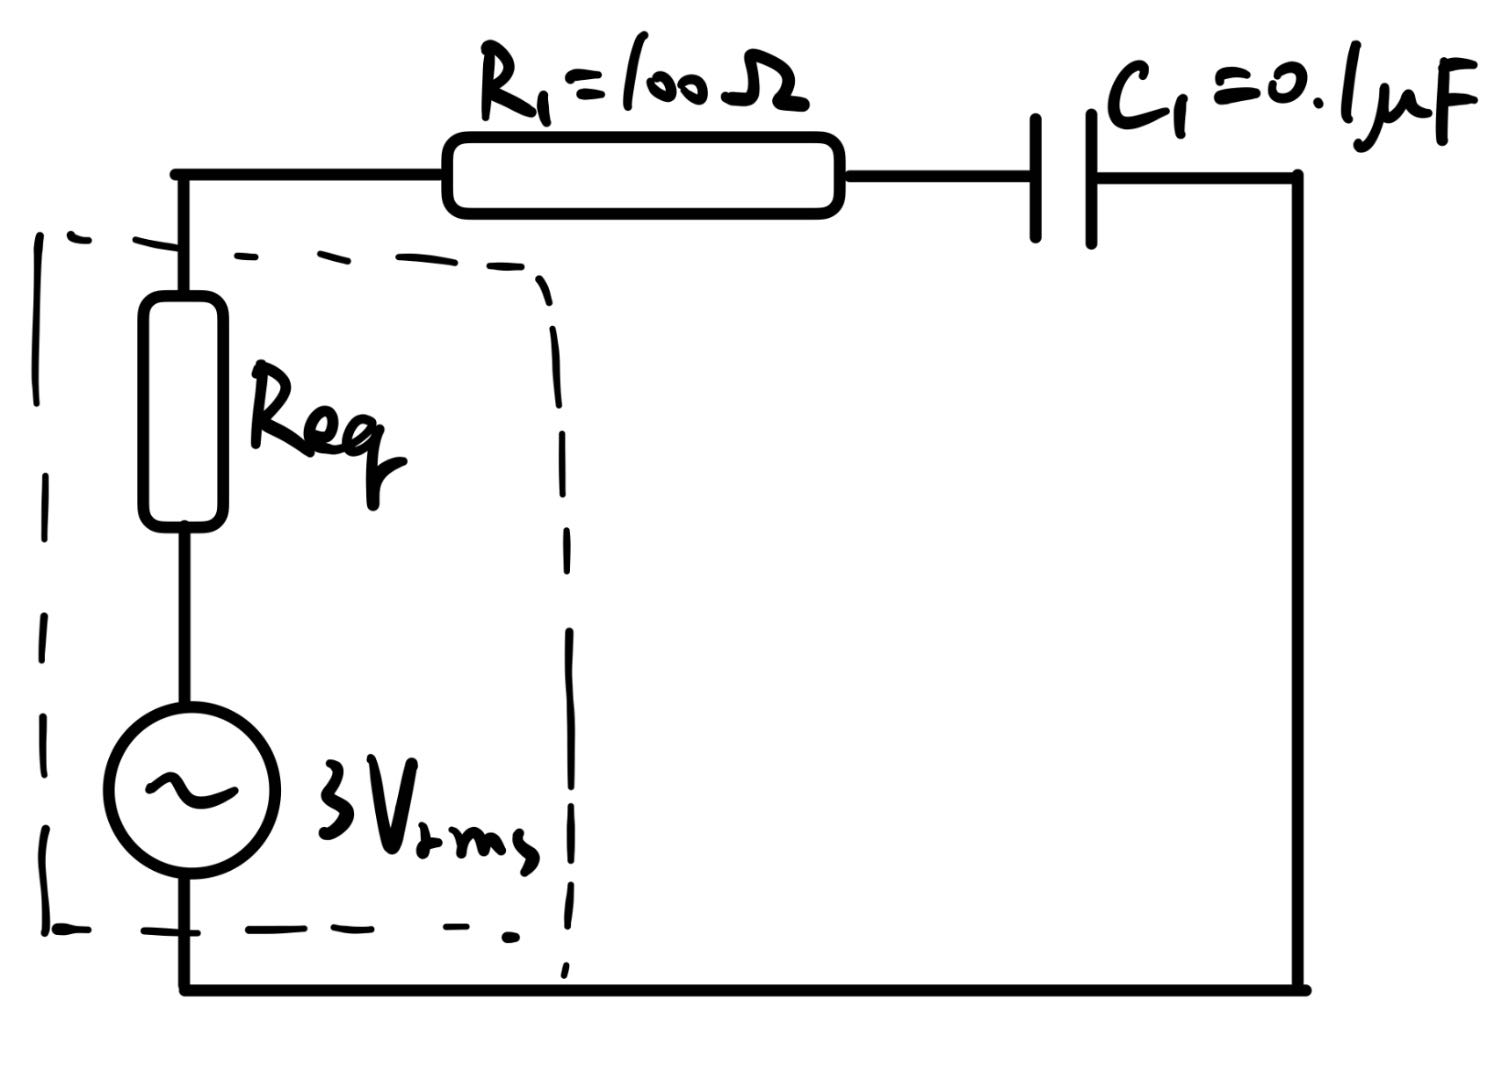
\includegraphics[width=0.35\textwidth]{graph2-1-1.jpg}\label{fig:graph2-1-1}}
				\quad
				\subfloat[RL电路的阻抗频率特性电路图]
				{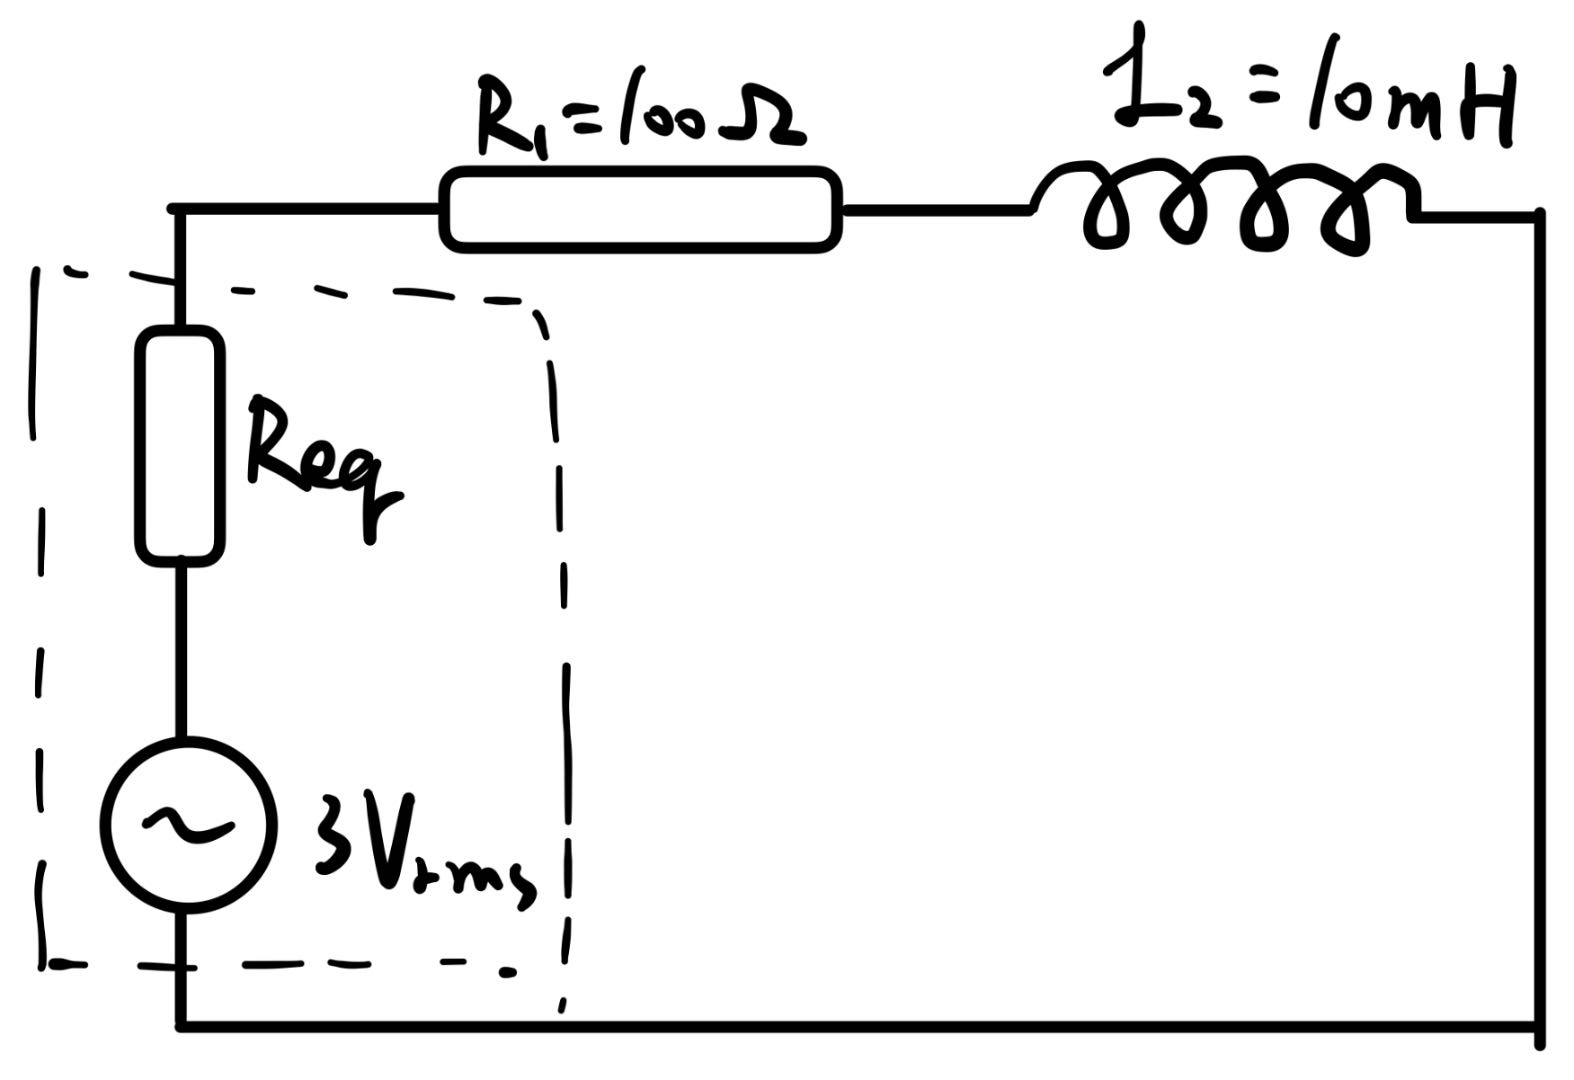
\includegraphics[width=0.35\textwidth]{graph2-1-2.jpg}\label{fig:graph2-1-2}}
				\quad				
				\caption{测量阻抗频率特性电路图}
				\label{fig:graph2-2}
			\end{figure}

		\begin{enumerate}
			\item 使信号源的输出频率从100Hz逐渐增至100KHz左右, 并使端点S分别接通R、L、C三个元件,分别测量 $U_R$ 、$U_r$ ,$U_L$、$U_r$,$U_C$、$U_r$,并通过计算得到\textbf{各频率点时的R、$X_L$与$X_C$之值}。
			
			\item 根据以上测试数据,绘制串联电路中电抗元件上电压的\textbf{幅频关系曲线}(详见数据分析部分)。
			
			\item 找到RL,RC串联电路中,电抗元件与电阻分压相等的频率点f1,并在这个频率点的两端,使得电阻与电抗分压约等于2:1和1:2的频率点f2f3,绘制在这些频率点上的\textbf{电压向量三角形}和\textbf{阻抗三角形}。
		\end{enumerate}
		
		\item 用双踪示波器观察RL串联和RC串联电路在不同频率下阻抗角的变化情况,记录数据,
		绘制\textbf{相频特性曲线}。测量在频率f1、f2、f3处的阻抗角,与电压向量三角形和阻抗三角形做比较。
		
		\item 实验中的电感L不是理想电感,请设计实验方案,测量出该电感内部包含的\textbf{自有电阻RL}并验证。
		
			实验方案:方案一是直接用欧姆表测量,方案二是利用测量幅频关系曲线的数据进行拟合,在拟合函数中加入参数RL,根据拟合结果作为RL测量值。分别用实验方案一与实验方案二测量得到结果如果相近,那么便得到了验证。
	\end{enumerate}	
	
	%
	\subsubsection{实验结果展示}
	\begin{enumerate}
		\item 测量R、L、C元件的阻抗频率特性
		
		按照实验方案(电路\cref{fig:graph2-2}),测量得到的数据如\cref{tab:tab4}和\cref{tab:tab5}所示。

		% \begin{table}[htbp]
		% 	\centering
		% 	\begin{minipage}{.5\linewidth}
		% 	  \centering
		% 	  \caption{RC电路的阻抗频率特性实验数据}
		% 		\begin{tabular}{|c|cc|} 
		% 			\hline
		% 			$\log(f/Hz)$ & $U_{R1}/V$ & $U_{C1}/V$  \\ 
		% 			\hline
		% 			2        & 0.0019  & 2.997    \\
		% 			2.3      & 0.038   & 2.997    \\
		% 			2.6      & 0.0757  & 2.995    \\
		% 			2.9      & 0.1505  & 2.988    \\
		% 			3.2      & 0.297   & 2.961    \\
		% 			3.5      & 0.572   & 2.867    \\
		% 			3.8      & 1.018   & 2.566    \\
		% 			4.1      & 1.517   & 1.923    \\
		% 			4.4      & 1.828   & 1.167    \\
		% 			4.7      & 1.947   & 0.627    \\
		% 			5        & 1.995   & 0.324    \\
		% 			\hline
		% 		\end{tabular}
		% 	  \label{tab:tab4}
		% 	\end{minipage}%
		% 	\begin{minipage}{.5\linewidth}
		% 	  \centering
		% 	  \caption{数据:数控恒流源的伏安特性}
		% 	  	\begin{tabular}{|c|c|c|}
		% 			\hline
		% 			Rx/Ω & U/mV & Ix/mA \\
		% 			\hline
		% 			0.1 & 0.12 & 1.21 \\
		% 			0.2 & 0.23 & 1.14 \\
		% 			0.3 & 0.33 & 1.11 \\
				
		% 			16000 & 13600.00 & 0.85 \\
		% 			\hline
		% 		\end{tabular}
		% 	  \label{tab:tab5}
		% 	\end{minipage}
			
			
		% \end{table}


				% \begin{table}[htbp]
				% 	\centering
				% 	\begin{minipage}{.5\linewidth}
				% 	  \centering
				% 	  \caption{RC电路的阻抗频率特性实验数据}
				% 		\begin{tabular}{|c|cc|} 
				% 			\hline
				% 			$\log(f/Hz)$ & $U_{R1}/V$ & $U_{C1}/V$  \\ 
				% 			\hline
				% 			2        & 0.0019  & 2.997    \\
				% 			2.3      & 0.038   & 2.997    \\
				% 			2.6      & 0.0757  & 2.995    \\
				% 			2.9      & 0.1505  & 2.988    \\
				% 			3.2      & 0.297   & 2.961    \\
				% 			3.5      & 0.572   & 2.867    \\
				% 			3.8      & 1.018   & 2.566    \\
				% 			4.1      & 1.517   & 1.923    \\
				% 			4.4      & 1.828   & 1.167    \\
				% 			4.7      & 1.947   & 0.627    \\
				% 			5        & 1.995   & 0.324    \\
				% 			\hline
				% 			\end{tabular}
				% 	  \label{tab:tab4}
				% 	\end{minipage}
					
				% 	\begin{minipage}{.5\linewidth}
				% 	  \centering
				% 	  \caption{RL电路的阻抗频率特性实验数据}
				% 		\begin{tabular}{|c|cc|} 
				% 			\hline
				% 			$\log(f/Hz)$ & $U_{R1}/V$ & $U_{L2}/V$  \\ 
				% 			\hline
				% 			2        & 1.795   & 0.318    \\
				% 			2.3      & 1.79    & 0.373    \\
				% 			2.6      & 1.774   & 0.535    \\
				% 			2.9      & 1.716   & 0.907    \\
				% 			3.2      & 1.534   & 1.552    \\
				% 			3.5      & 1.15    & 2.286    \\
				% 			3.8      & 0.697   & 2.75     \\
				% 			4.1      & 0.366   & 2.928    \\
				% 			4.4      & 0.169   & 2.982    \\
				% 			4.7      & 0.046   & 3.001    \\
				% 			5        & 0.055   & 3.029    \\
				% 			\hline
				% 			\end{tabular}
				% 	  \label{tab:tab5}
				% 	\end{minipage}					
					
				% \end{table}


				\begin{table}[htbp]
					\begin{minipage}{.5\linewidth}
					  \centering
					  \caption{RC电路的阻抗频率特性实验数据}
					  \begin{tabular}{|c|cc|} 
						  \hline
						  $\log(f/Hz)$ & $U_{R1}/V$ & $U_{C1}/V$  \\ 
						  \hline
						  2        & 0.0019  & 2.997    \\
						  2.3      & 0.038   & 2.997    \\
						  2.6      & 0.0757  & 2.995    \\
						  2.9      & 0.1505  & 2.988    \\
						  3.2      & 0.297   & 2.961    \\
						  3.5      & 0.572   & 2.867    \\
						  3.8      & 1.018   & 2.566    \\
						  4.1      & 1.517   & 1.923    \\
						  4.4      & 1.828   & 1.167    \\
						  4.7      & 1.947   & 0.627    \\
						  5        & 1.995   & 0.324    \\
						  \hline
					  \end{tabular}
					  \label{tab:tab4}
					\end{minipage}%
					\begin{minipage}{.5\linewidth}
					  \centering
					  \caption{RL电路的阻抗频率特性实验数据}
					  \begin{tabular}{|c|cc|} 
						  \hline
						  $\log(f/Hz)$ & $U_{R1}/V$ & $U_{L2}/V$  \\ 
						  \hline
						  2        & 1.795   & 0.318    \\
						  2.3      & 1.79    & 0.373    \\
						  2.6      & 1.774   & 0.535    \\
						  2.9      & 1.716   & 0.907    \\
						  3.2      & 1.534   & 1.552    \\
						  3.5      & 1.15    & 2.286    \\
						  3.8      & 0.697   & 2.75     \\
						  4.1      & 0.366   & 2.928    \\
						  4.4      & 0.169   & 2.982    \\
						  4.7      & 0.046   & 3.001    \\
						  5        & 0.055   & 3.029    \\
						  \hline
					  \end{tabular}
					  \label{tab:tab5}
					\end{minipage}
				\end{table}
				
		
		\item 测量特定频率下的阻抗三角形与电压三角形
		
		电压三角形:
		
		按照实验方案(电路\cref{fig:graph2-2}),测量得到的数据如\cref{tab-RC}和\cref{tab-RL}所示。

		\begin{table}
			\centering
			\begin{tblr}{
			  cells = {c},
			  vline{1-2,6} = {-}{},
			  hline{1-2,5} = {-}{},
			}
				   & 理论值     & 实际值     & UR      & UL    \\
			1:1分压时 & 1592.35 & 1565.96 & 1.539   &       \\
			1:2分压时 & 3183.1  & 3183.1  & 1.14514 & 2.292 \\
			2:1分压时 & 759.775 & 746.1   & 1.724   & 0.826 
			\end{tblr}
			\caption{RC电路的阻抗频率特性特殊点实验数据}
			\label{tab-RC}
		\end{table}

		\begin{table}
			\centering
			\begin{tblr}{
			  cells = {c},
			  vline{1-2,6} = {-}{},
			  hline{1-2,5} = {-}{},
			}
				   & 理论值     & 实际值     & UR    & UL    \\
			1:1分压时 & 15915.5 & 15975.5 & 1.652 &       \\
			1:2分压时 & 7957.75 & 7957.75 & 1.193 & 2.387 \\
			2:1分压时 & 3183.1  & 3213.1  & 1.886 & 0.944 
			\end{tblr}
			\caption{RL电路的阻抗频率特性特殊点实验数据}
			\label{tab-RL}
		\end{table}

		阻抗三角形:

		按照实验方案(电路\cref{fig:graph2-2}),测量得到的数据如\cref{table:tbl-impedence}所示。

% \usepackage{tabularray}
			\begin{table}
				\centering
				\begin{tblr}{
				cells = {c},
				cell{1}{1} = {r=4}{},
				cell{1}{4} = {r=4}{},
				vline{1,4,7} = {1}{},
				vline{1,4,7} = {2-4}{},
				hline{1,5} = {-}{},
				}
				RL相频 &        & $\Delta\phi$ & RC相频 &        & $\Delta\phi$ \\
					& 1:1分压时 & -8.274                       &      & 1:1分压时 & 5.443                                        \\
					& 1:2分压时 & -7.128                       &      & 1:2分压时 & 12.45                                        \\
					& 2:1分压时 & -1.603                       &      & 2:1分压时 & 13.43                                        
				\end{tblr}
				\caption{阻抗三角形实验数据}
				\label{table:tbl-impedence}
			\end{table}
		

		
		\item 测量相频特性
		
		按照实验方案(电路\cref{fig:graph2-2}),测量得到的数据如\cref{tab:tab6}和\cref{tab:tab7}所示。

			% \begin{table}[htbp]
			% 	\centering
			% 	\begin{minipage}{.5\linewidth}
			% 	  \centering
			% 	  \caption{RC电路的相频特性实验数据}
			% 		\begin{tblr}{
			% 			cells = {c},
			% 			vline{1,3} = {-}{},
			% 			hline{1-2,12} = {-}{},
			% 			}
			% 			$f/Hz$      & $\Delta\phi$     \\
			% 			100    & -1.8   \\
			% 			300    & -2.156 \\
			% 			600    & 4.046  \\
			% 			1000   & 5.4    \\
			% 			3000   & 9.7    \\
			% 			6000   & 24.91  \\
			% 			10000  & 28.14  \\
			% 			30000  & 59.33  \\
			% 			60000  & 79.15  \\
			% 			100000 & 79.3   
			% 		\end{tblr}
			% 	  \label{tab:tab6}
			% 	\end{minipage}%
				
			% 	\begin{minipage}{.5\linewidth}
			% 	  \centering
			% 	  \caption{RL电路的相频特性实验数据}
			% 			\begin{tabular}{|cc|} 
			% 				\hline
			% 				$f/Hz$       & $\Delta\phi$      \\ 
			% 				\hline
			% 				100    & -21.8   \\
			% 				300    & -41.2   \\
			% 				600    & -46.3   \\
			% 				1000   & -48.12  \\
			% 				3000   & -24.9   \\
			% 				6000   & -22.19  \\
			% 				10000  & -14.82  \\
			% 				30000  & 3.24    \\
			% 				60000  & -2.497  \\
			% 				100000 & 4.246   \\
			% 				\hline
			% 			\end{tabular}
			% 	  \label{tab:tab7}
			% 	\end{minipage}
				
				
			% \end{table}



			\begin{table}[htbp]
				\begin{minipage}{.5\linewidth}
				  \centering
				  \caption{RC电路的相频特性实验数据}
				  \begin{tblr}{
					  cells = {c},
					  vline{1,3} = {-}{},
					  hline{1-2,12} = {-}{},
					  }
					  $f$/Hz      & $\Delta\phi$     \\
					  100    & -1.8   \\
					  300    & -2.156 \\
					  600    & 4.046  \\
					  1000   & 5.4    \\
					  3000   & 9.7    \\
					  6000   & 24.91  \\
					  10000  & 28.14  \\
					  30000  & 59.33  \\
					  60000  & 79.15  \\
					  100000 & 79.3   
				  \end{tblr}
				  \label{tab:tab6}
				\end{minipage}%
				\begin{minipage}{.5\linewidth}
				  \centering
				  \caption{RL电路的相频特性实验数据}
				  \begin{tblr}{
					  cells = {c},
					  vline{1,3} = {-}{},
					  hline{1-2,12} = {-}{},
					  }
					  $f$/Hz       & $\Delta\phi$      \\ 
					  100    & -21.8   \\
					  300    & -41.2   \\
					  600    & -46.3   \\
					  1000   & -48.12  \\
					  3000   & -24.9   \\
					  6000   & -22.19  \\
					  10000  & -14.82  \\
					  30000  & 3.24    \\
					  60000  & -2.497  \\
					  100000 & 4.246   \\
				  \end{tblr}
				  \label{tab:tab7}
				\end{minipage}
			\end{table}
			
		
		
		
		\item 测量电感元件的自有电阻
		
		由实验方案一,测量$R_L=16.5\Omega$;由实验方案二,测量$R_L=7\omega$;至少在量级上,
		我们可以认为两个方案测量得到的结果差异不大。 
	\end{enumerate}
	
	
	% ---
	
	% 原始数据
	\clearpage
	\subsection{原始数据记录}
	实验记录本上的原始数据见\cref{fig:data1},\cref{fig:data2},\cref{fig:data3}(签字),\cref{fig:data4}。

	\begin{figure}[htbp]
		\centering
		\subfloat[原始数据1]
		{\includegraphics[width=0.3\textwidth]{ET1_6Gradata-1.jpg}\label{fig:data1}}
		\quad
		\subfloat[原始数据2]
		{\includegraphics[width=0.3\textwidth]{ET1_6Gradata-2.jpg}\label{fig:data2}}
		\quad
		\subfloat[原始数据3]
		{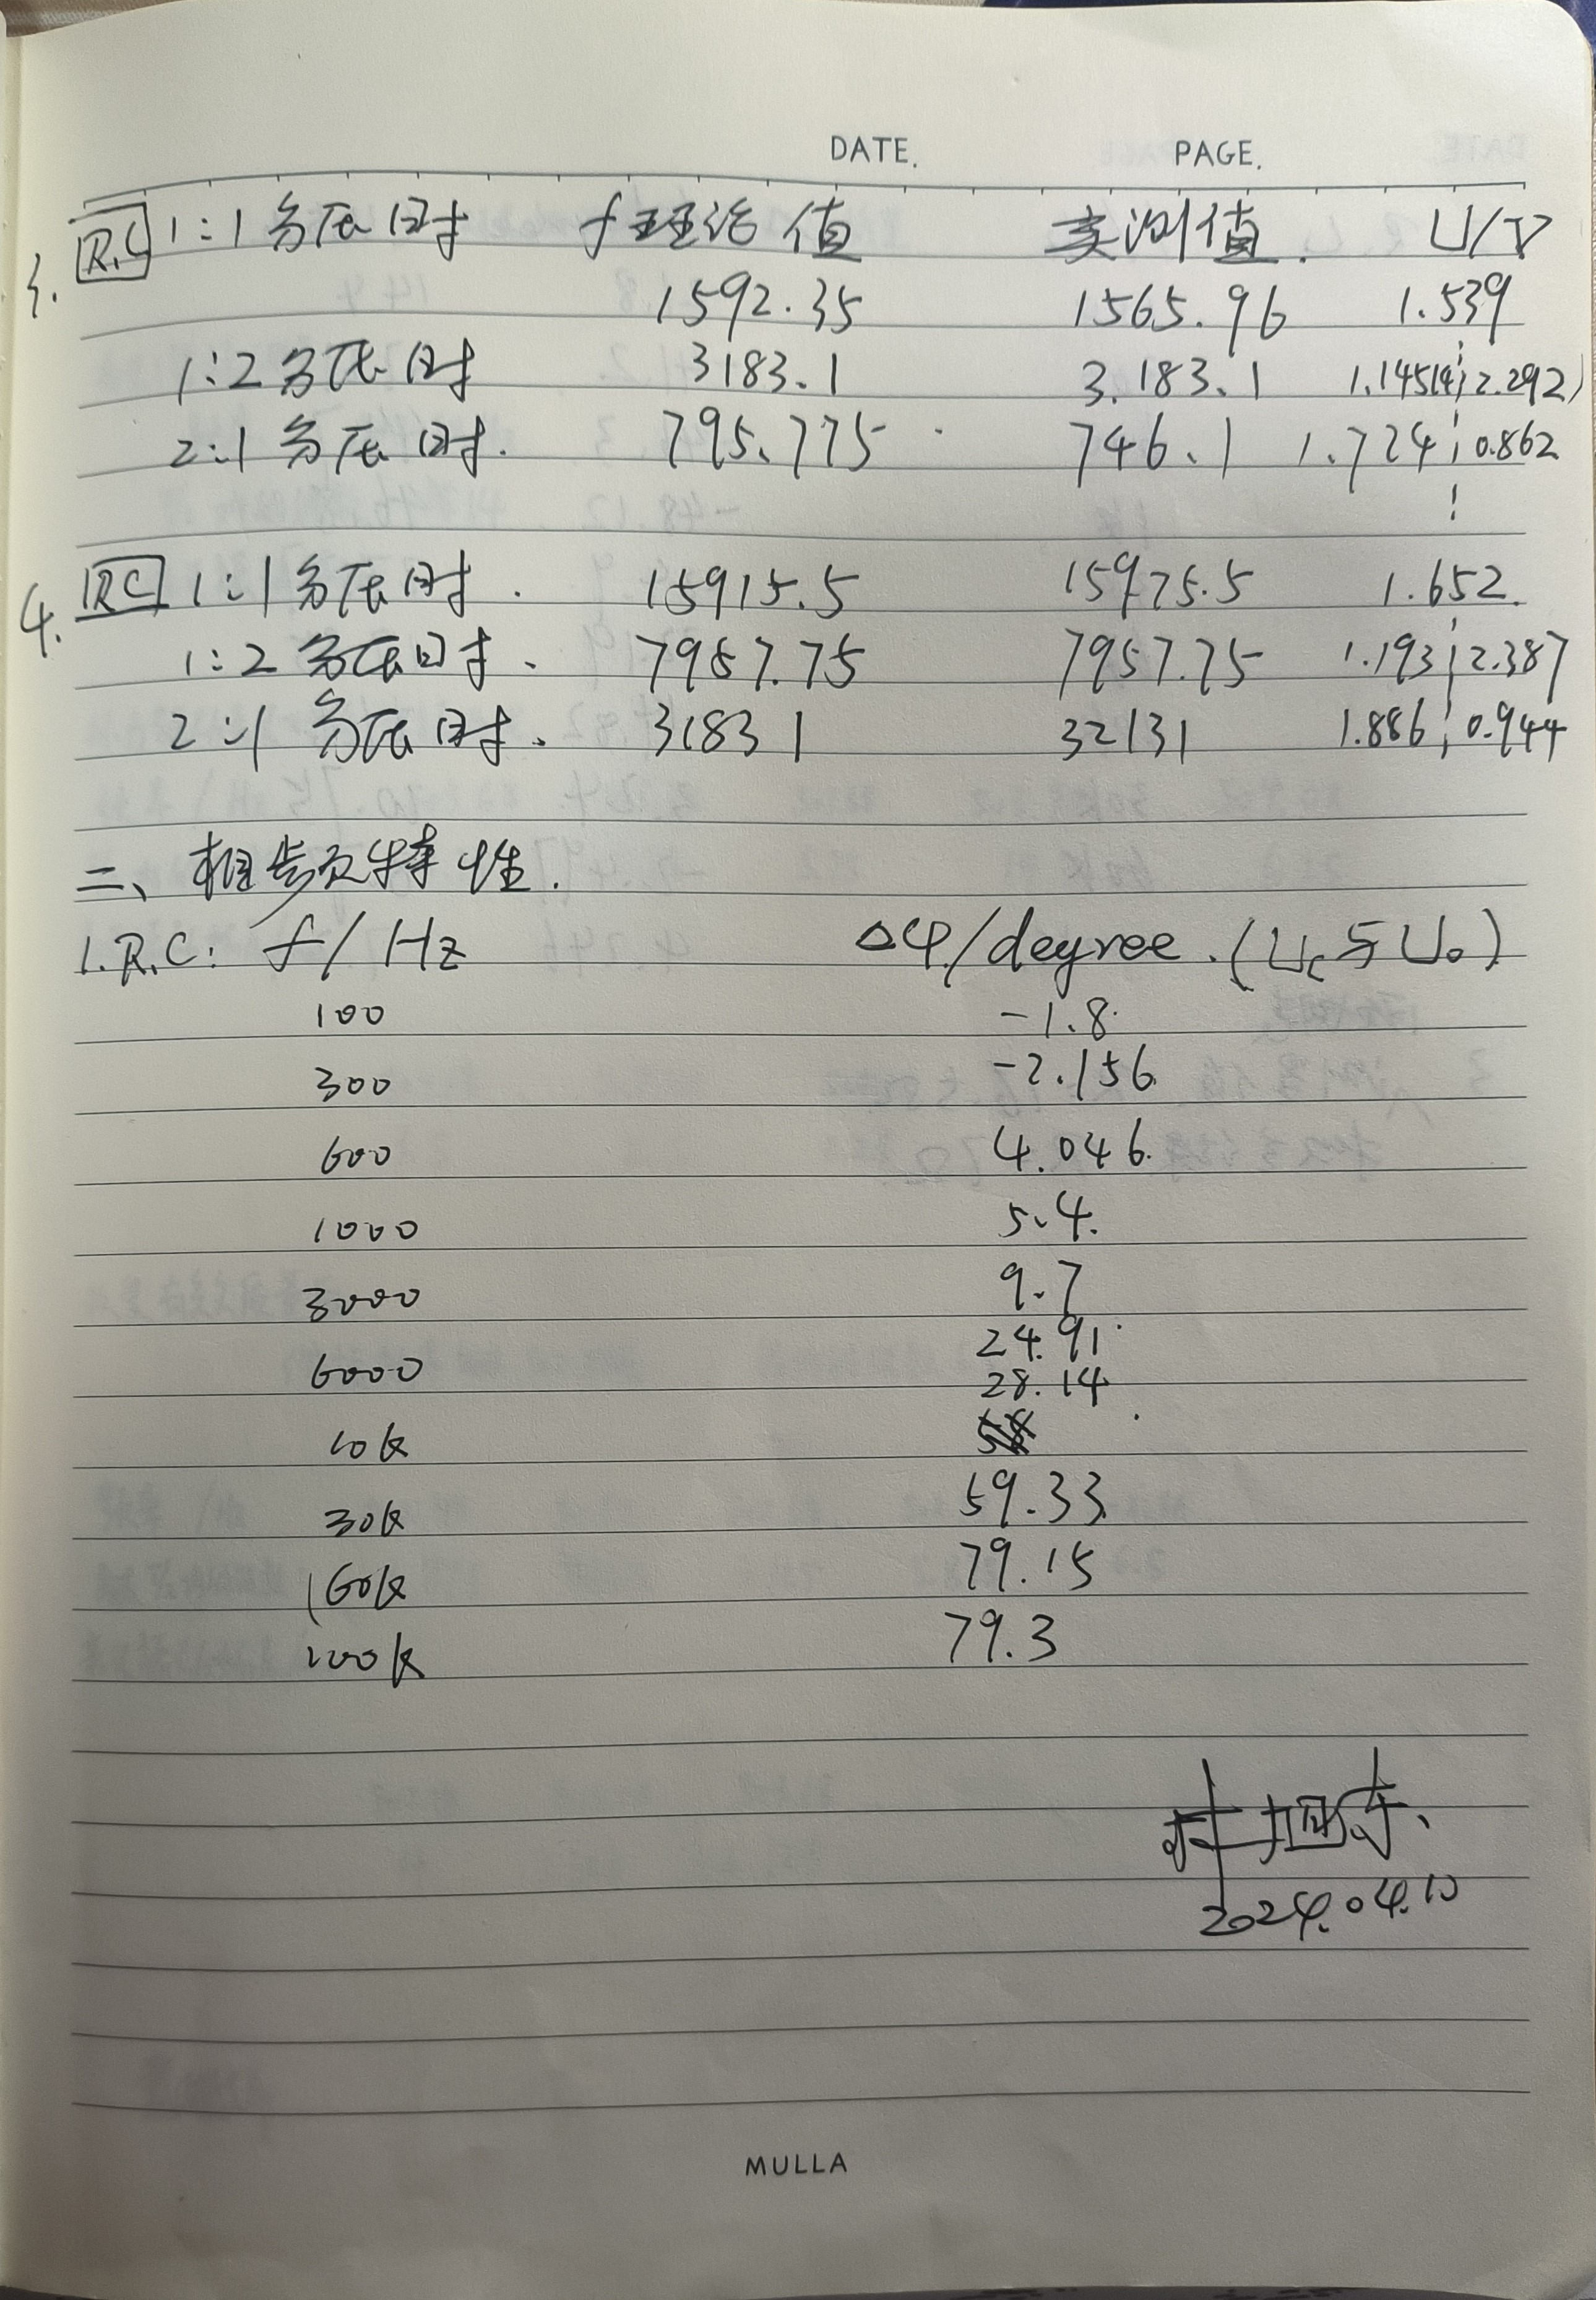
\includegraphics[width=0.3\textwidth]{ET1_6Gradata-3.jpg}\label{fig:data3}}
		\quad
		\subfloat[原始数据4]
		{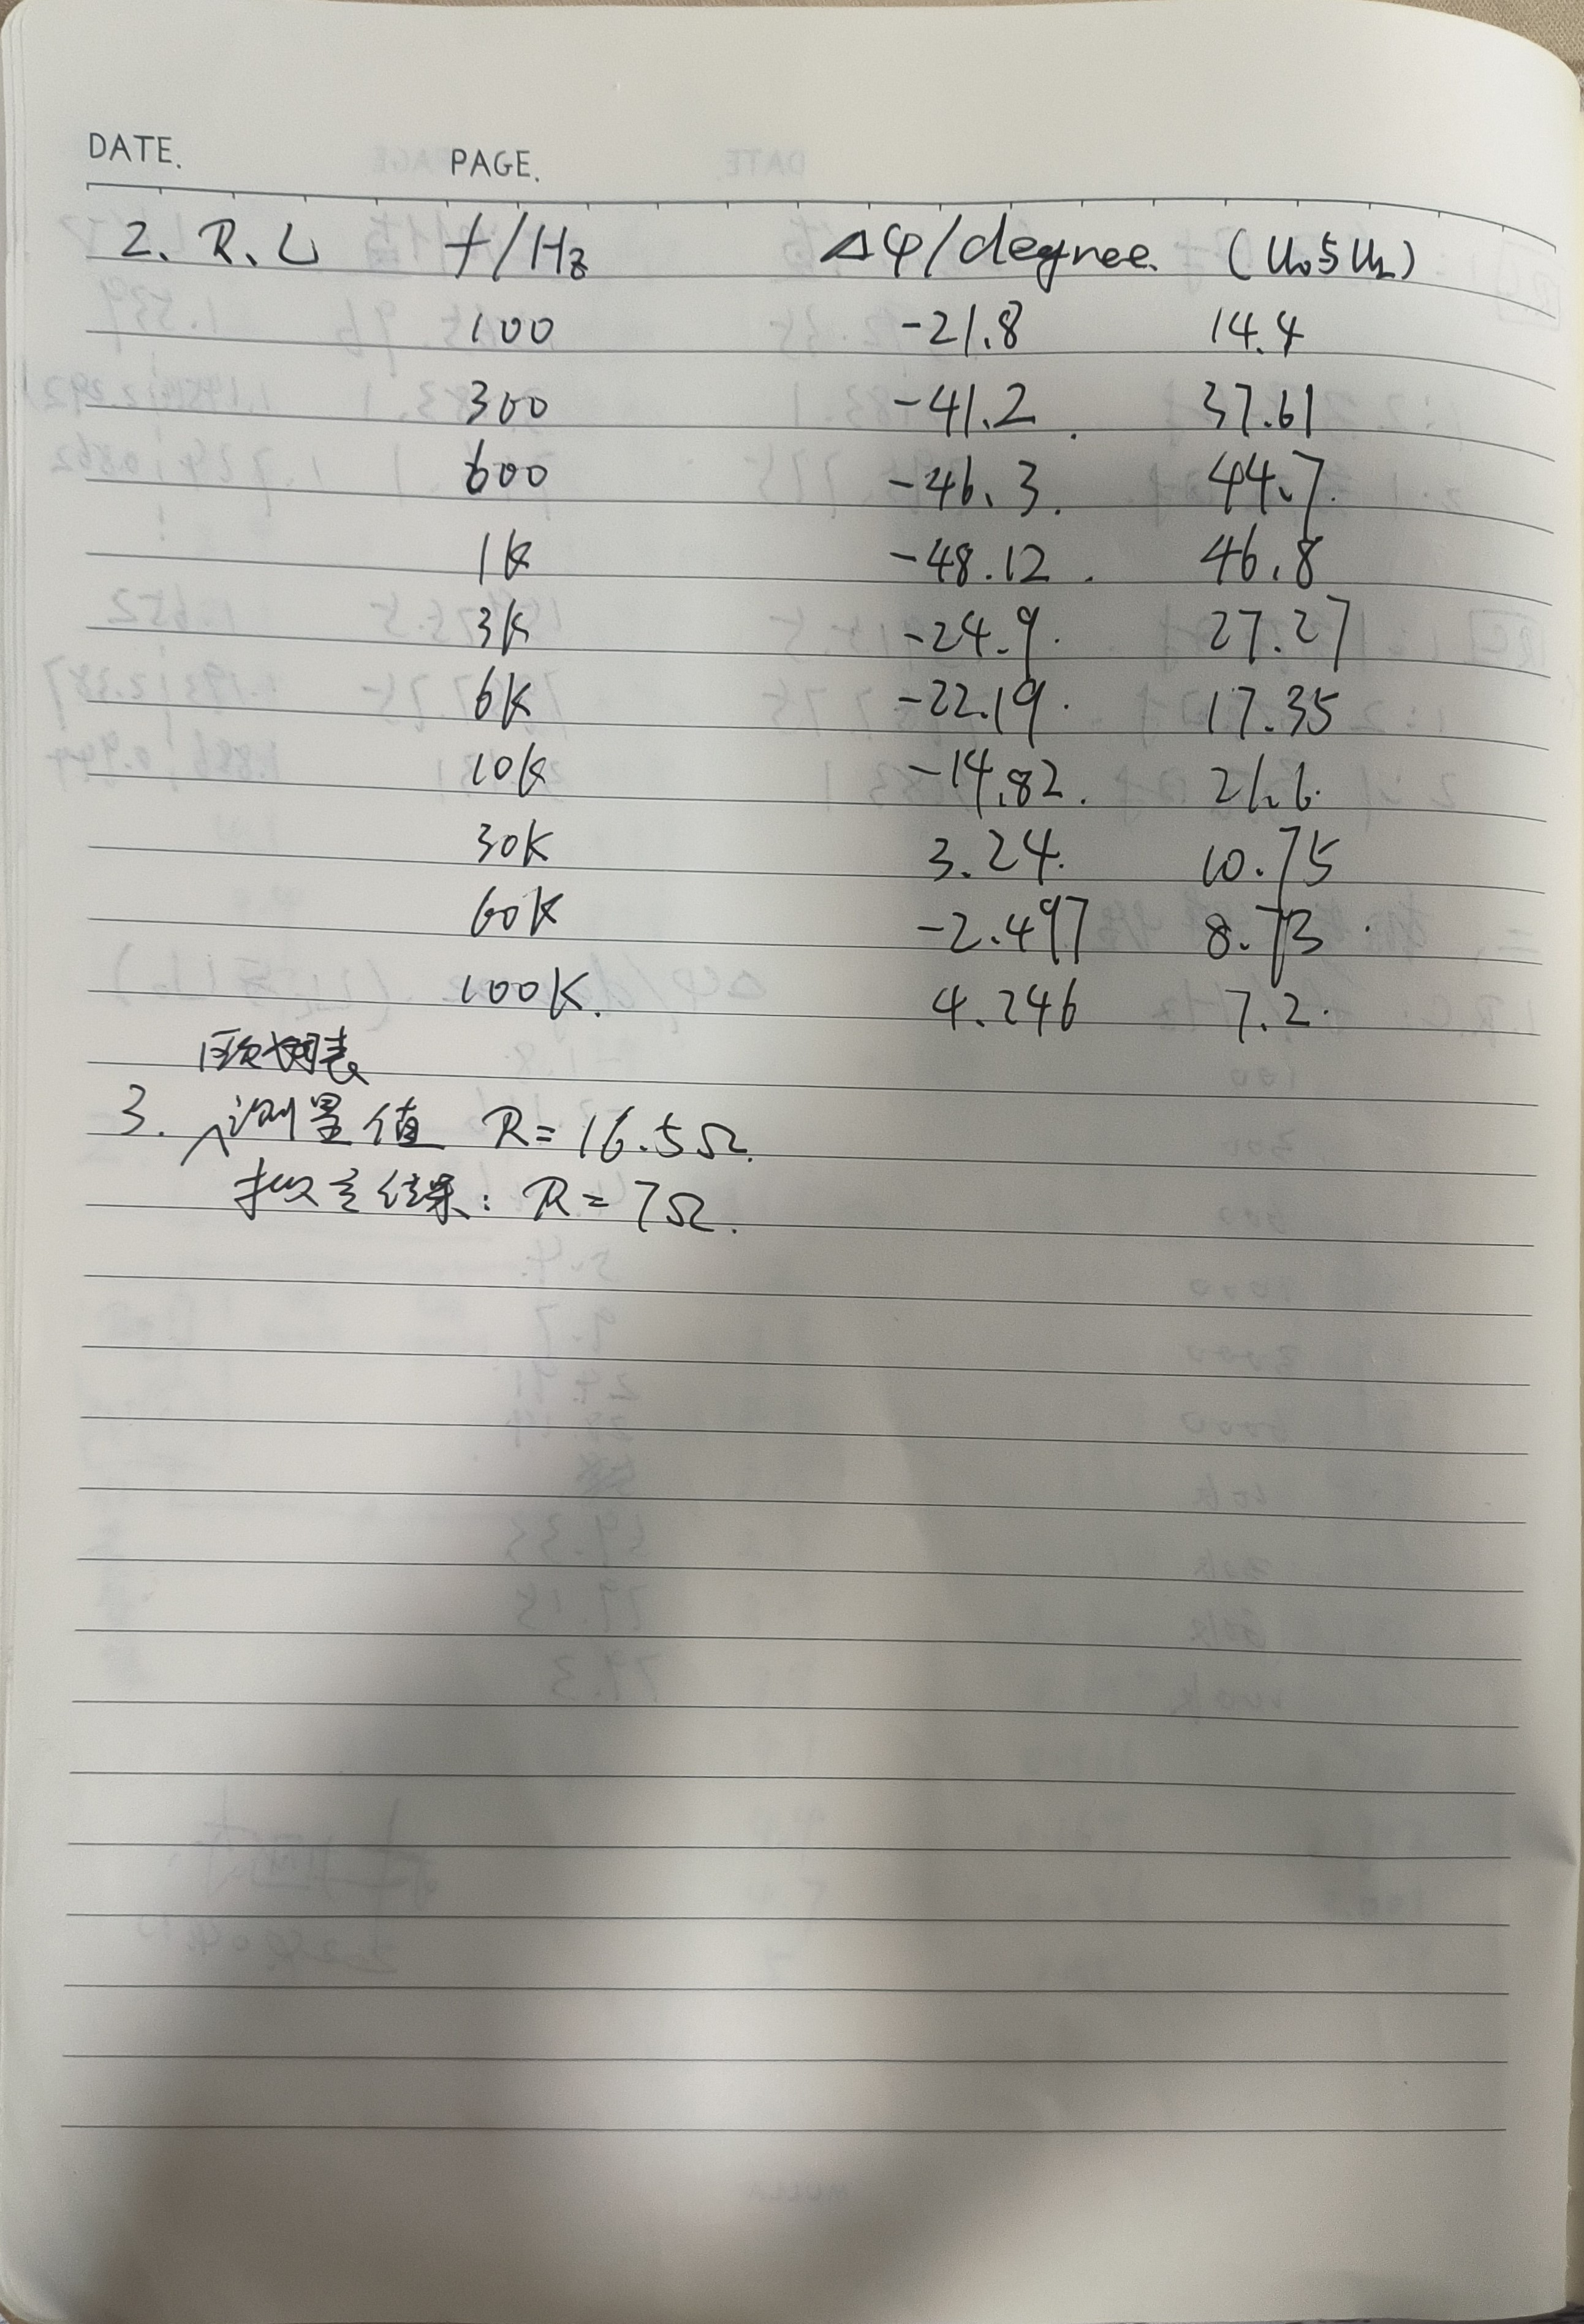
\includegraphics[width=0.3\textwidth]{ET1_6Gradata-4.jpg}\label{fig:data4}}
		\quad

		\caption{原始数据}
		\label{fig:original_data}
	\end{figure}
	
	%实验台桌面整理见%\textbf{附件}部分(\cref{})。
	
	%其它原始数据见%\cref{}。
	% ---
	
	% 问题记录
	%\subsection{实验过程遇到问题及解决办法}
	
	% ---
	
	
	
	% 分析与讨论	
	\clearpage
	
	% 顶栏
	\begin{table}
		\renewcommand\arraystretch{1.7}
		\begin{tabularx}{\textwidth}{|X|X|X|X|}
			\hline
			专业:& 物理学 &年级:& 2022级\\
			\hline
			姓名: & 戴鹏辉、杨舒云 & 学号:& 22344016、22344020\\
			\hline
			日期:& 2024/4/10 & 评分: &\\
			\hline
		\end{tabularx}
	\end{table}
	% ---
	
	% 小标题
	\section{ET1-6\quad R、L、C元件阻抗特性研究 \quad\heiti 分析与讨论}
	% ---
	
	% 数据处理
	\subsection{实验数据分析}
	
	%
	\subsubsection{R、L、C元件的阻抗频率特性}
	\begin{enumerate}
		\item 验证数据与考虑发生器内阻
		
		引入前面在戴维南定理相关实验中测定的数据,我们可以进行如\cref{tab:tab29}和\cref{tab:tab30}所示的分析。
		
		\begin{table}[h]
			\centering
			\caption{频率对应的电压和计算值}
			\label{tab:tab29}
			\begin{tabular}{|c|c|c|c|c|}
				\hline
				$lg(f/Hz)$ & $U_{R1}/V$ & $U_{C1}/V$ & $U_R/V$ & $U_R^2+U_{C1}^2$ \\
				\hline
				2 & 0.0019 & 2.997 & 0.002888 & 8.982017341 \\
				2.3 & 0.038 & 2.997 & 0.05776 & 8.985345218 \\
				2.6 & 0.0757 & 2.995 & 0.115064 & 8.983264724 \\
				2.9 & 0.1505 & 2.988 & 0.22876 & 8.980475138 \\
				3.2 & 0.297 & 2.961 & 0.45144 & 8.971319074 \\
				3.5 & 0.572 & 2.867 & 0.86944 & 8.975614914 \\
				3.8 & 1.018 & 2.566 & 1.54736 & 8.97867897 \\
				4.1 & 1.517 & 1.923 & 2.30584 & 9.014827106 \\
				4.4 & 1.828 & 1.167 & 2.77856 & 9.082284674 \\
				4.7 & 1.947 & 0.627 & 2.95944 & 9.151414114 \\
				5 & 1.995 & 0.324 & 3.0324 & 9.30042576 \\
				\hline
			\end{tabular}
		\end{table}
		
		\begin{table}[h]
			\centering
			\caption{频率对应的电压和计算值}
			\label{tab:tab30}
			\begin{tabular}{|c|c|c|c|c|}
				\hline
				lg(f/Hz) & $U_{R1}/V$ & $U_{L2}/V$ & $U_R/V$ & $U_R^2+U_{L2}^2$ \\
				\hline
				2 & 1.795 & 0.318 & 3.03355 & 9.303549603 \\
				2.3 & 1.79 & 0.373 & 3.043 & 9.398978 \\
				2.6 & 1.774 & 0.535 & 3.0158 & 9.38127464 \\
				2.9 & 1.716 & 0.907 & 2.9172 & 9.33270484 \\
				3.2 & 1.534 & 1.552 & 2.6078 & 9.20932484 \\
				3.5 & 1.15 & 2.286 & 1.955 & 9.047821 \\
				3.8 & 0.697 & 2.75 & 1.1849 & 8.96648801 \\
				4.1 & 0.366 & 2.928 & 0.6222 & 8.96031684 \\
				4.4 & 0.169 & 2.982 & 0.2873 & 8.97486529 \\
				4.7 & 0.046 & 3.001 & 0.0782 & 9.01211624 \\
				5 & 0.055 & 3.029 & 0.0935 & 9.18358325 \\
				\hline
			\end{tabular}
		\end{table}		
		
		可见在引入合理的信号源内阻后,测量结果能非常自洽地吻合。	
		
		\item 计算阻抗,讨论阻抗频率特性
		
		由测量得到的数据计算得到阻抗,并作出阻抗频率特性如\cref{fig:figC1}和\cref{fig:figC2}所示。
		
		\begin{figure}[htbp]
			\centering
			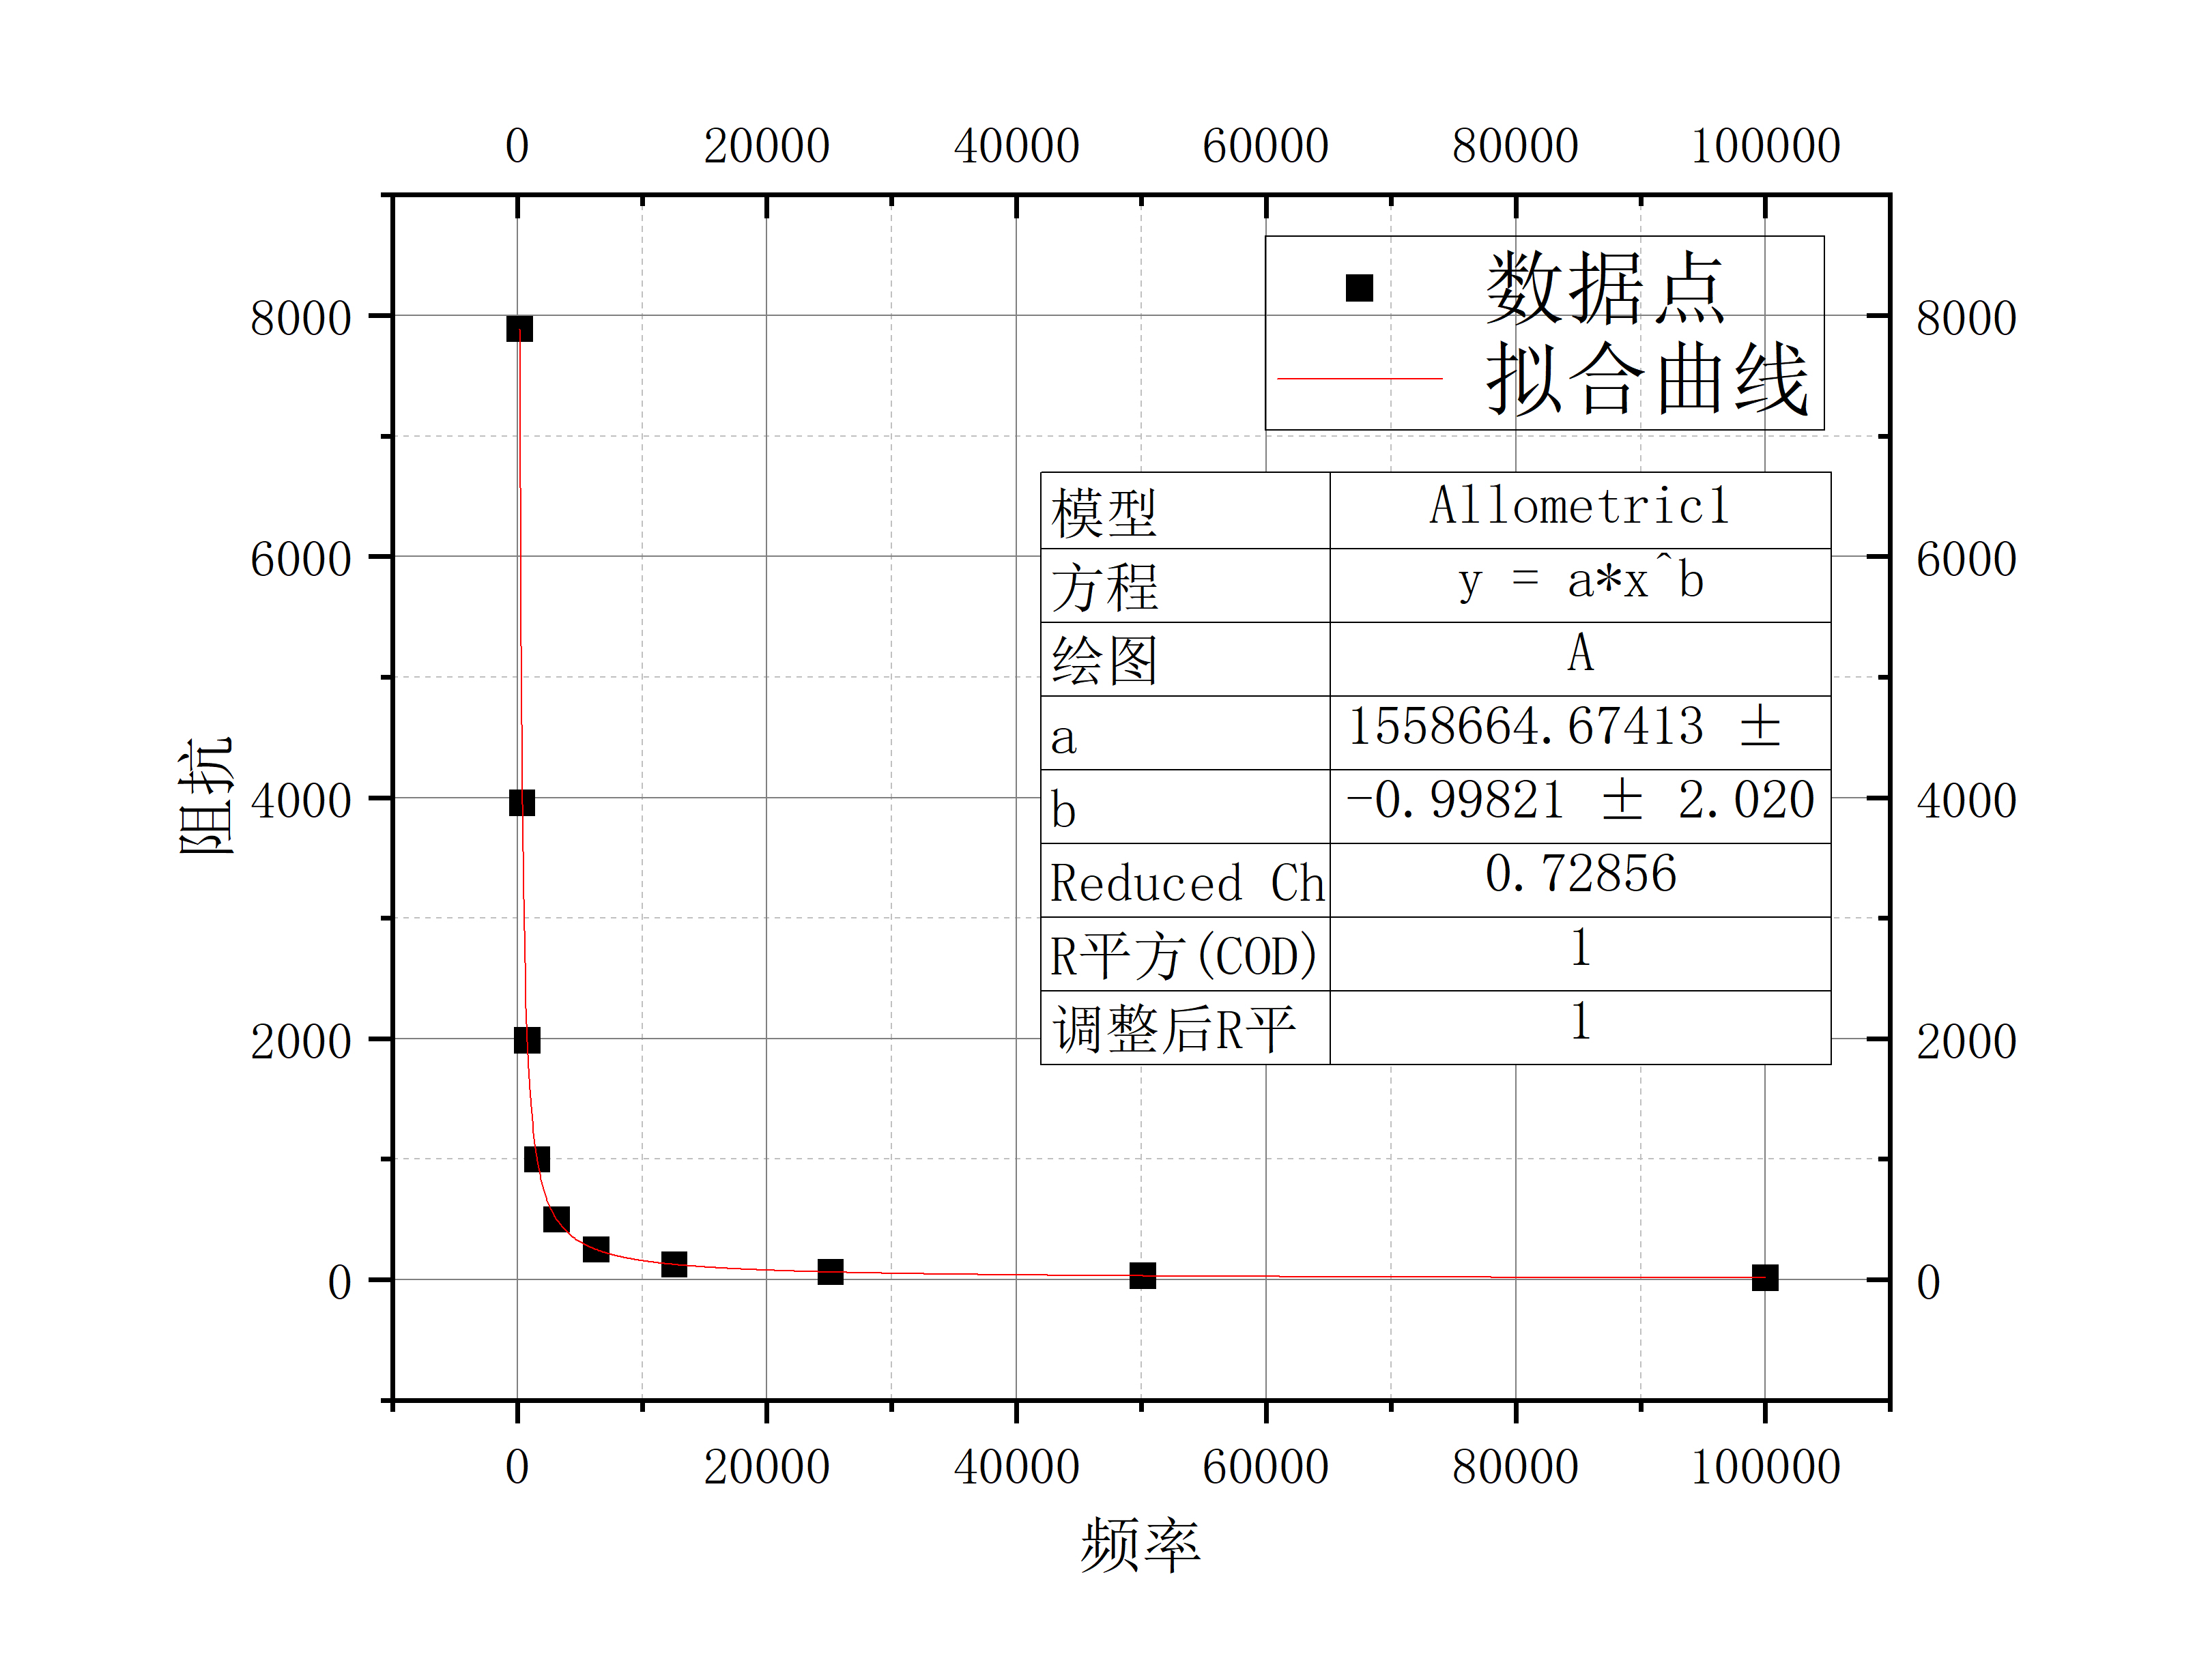
\includegraphics[width=0.5\textwidth]{ET1_6GraC1.jpg}
			\caption{C阻抗频率特性}
			\label{fig:figC1}
		\end{figure}
		
		\begin{figure}[htbp]
			\centering
			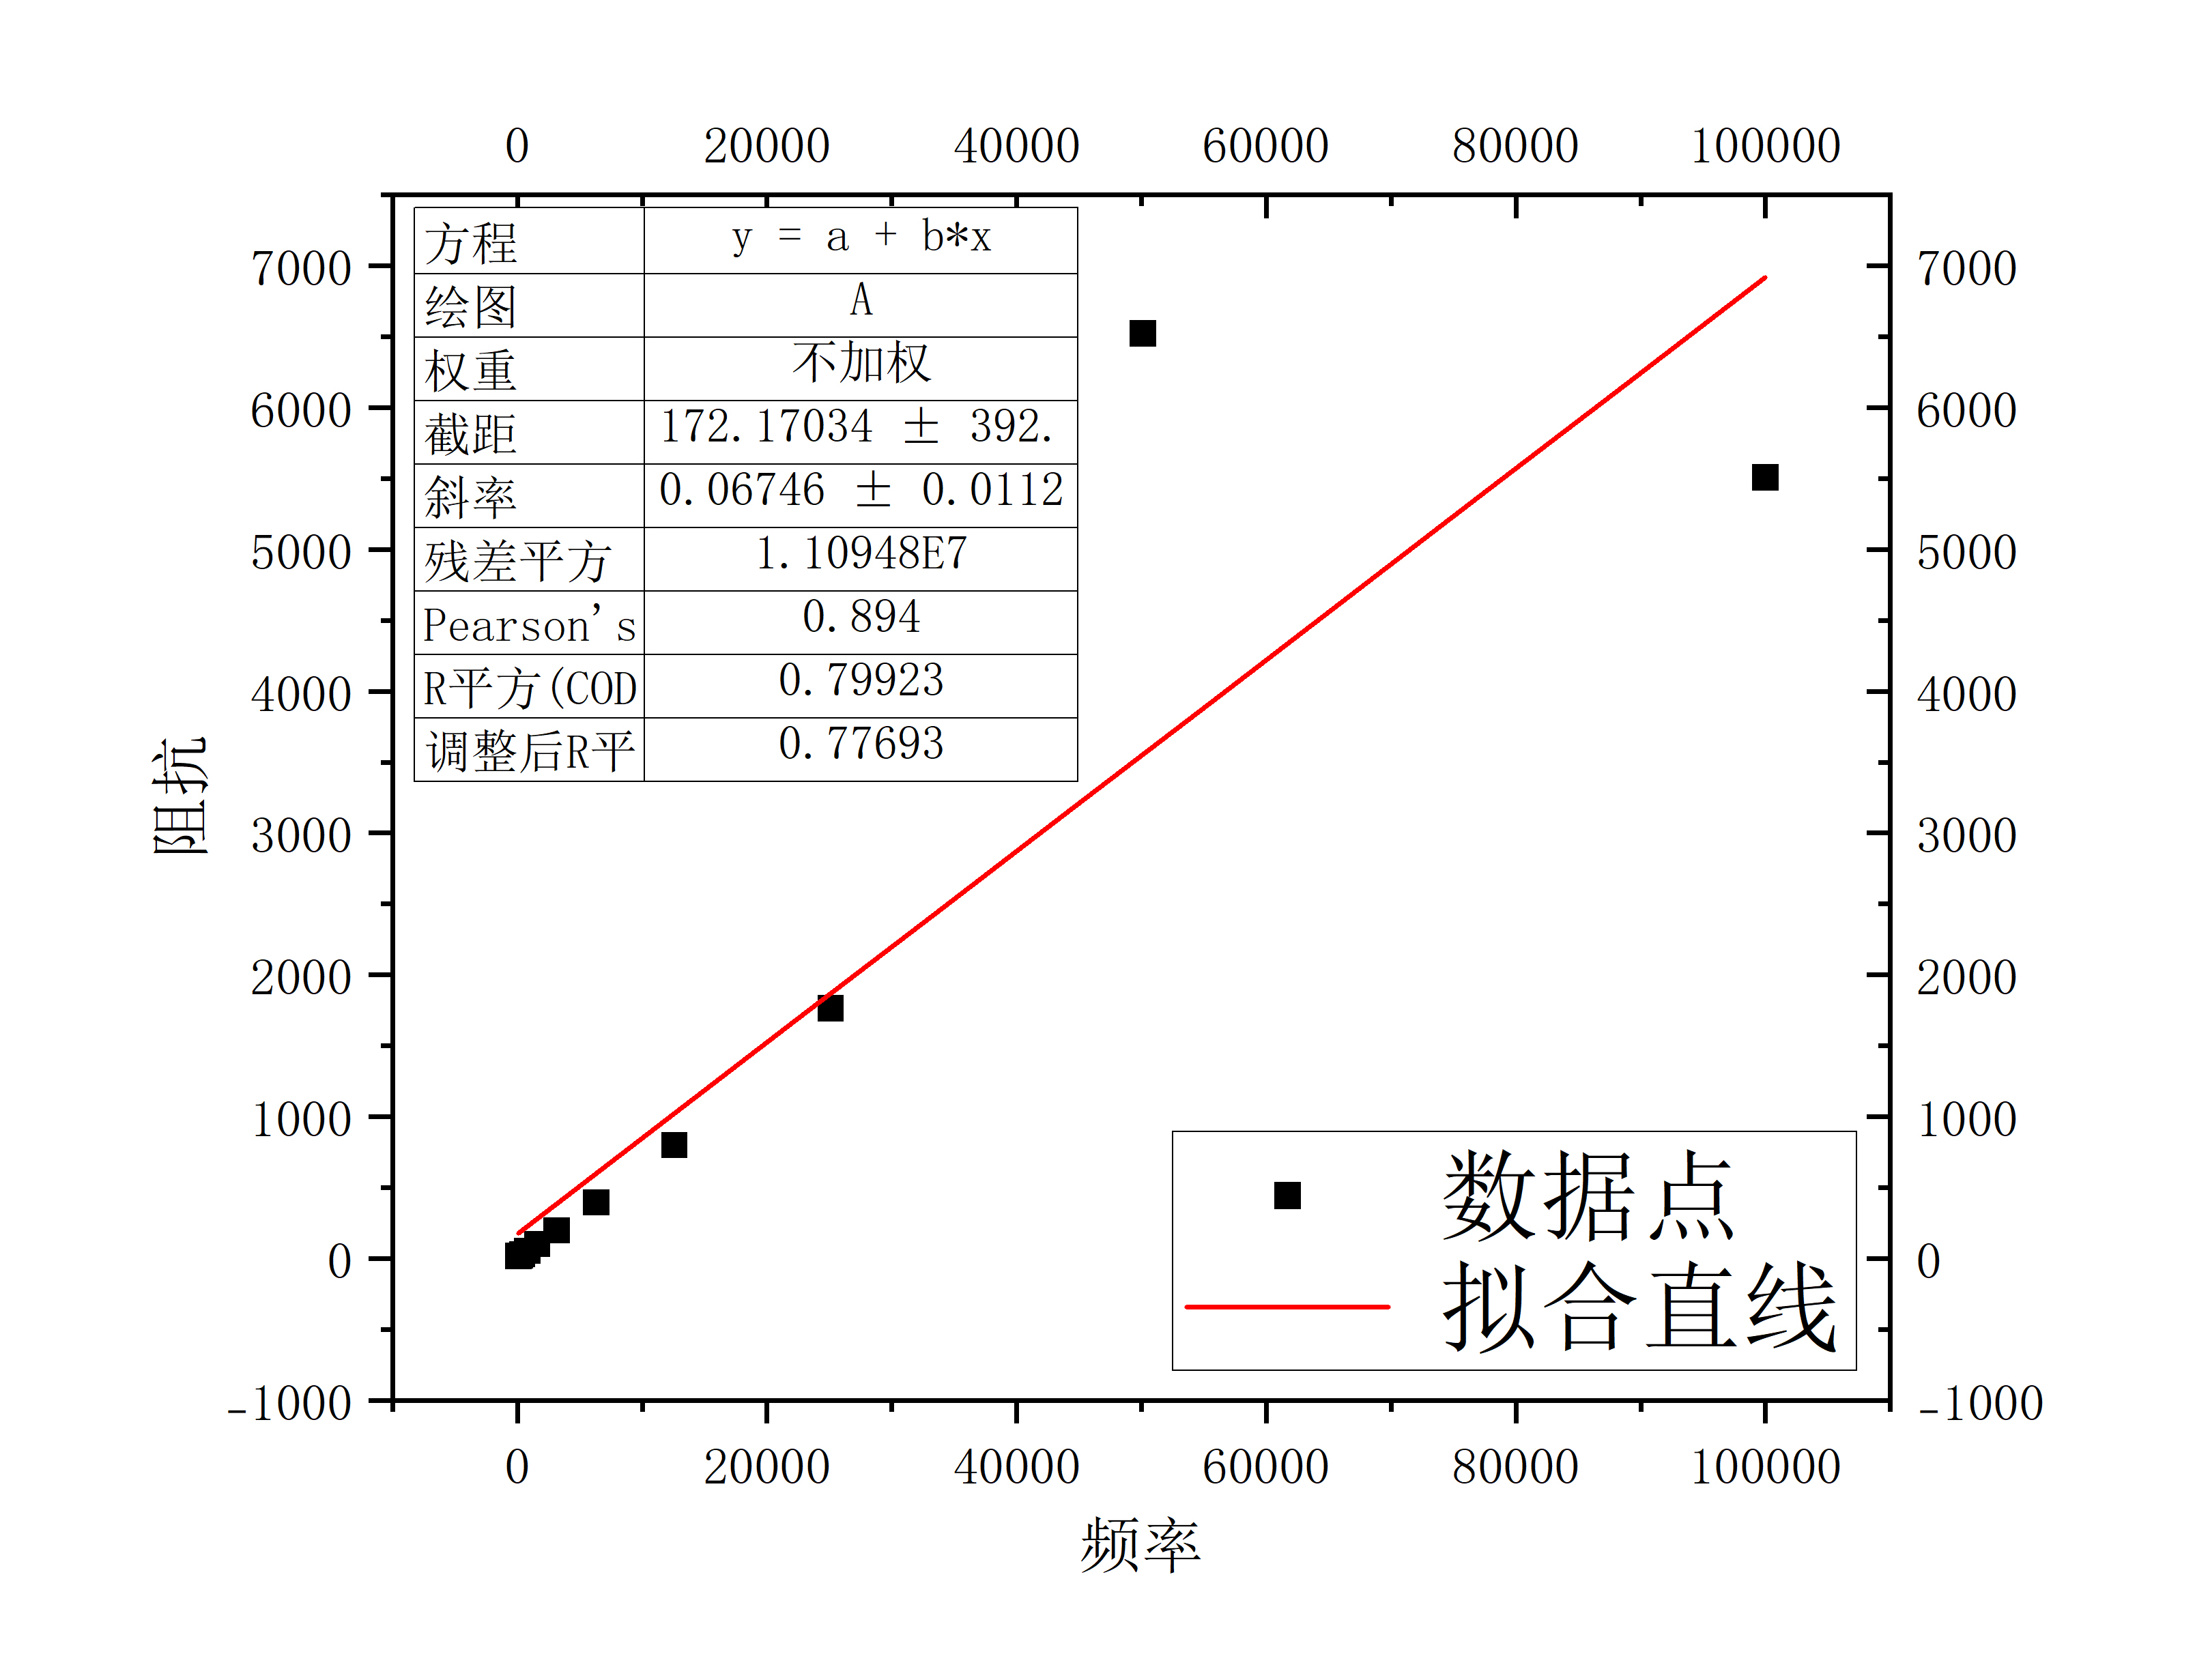
\includegraphics[width=0.5\textwidth]{ET1_6GraC2.jpg}
			\caption{L阻抗频率特性}
			\label{fig:figC2}
		\end{figure}
		
		\item 电压向量三角形
		
			先讨论RC电路的电压向量三角形:

			由\cref{tab-RC}可得到如下图像\cref{fig:graph3-1-1}

			\begin{figure}[htbp]
				\centering
				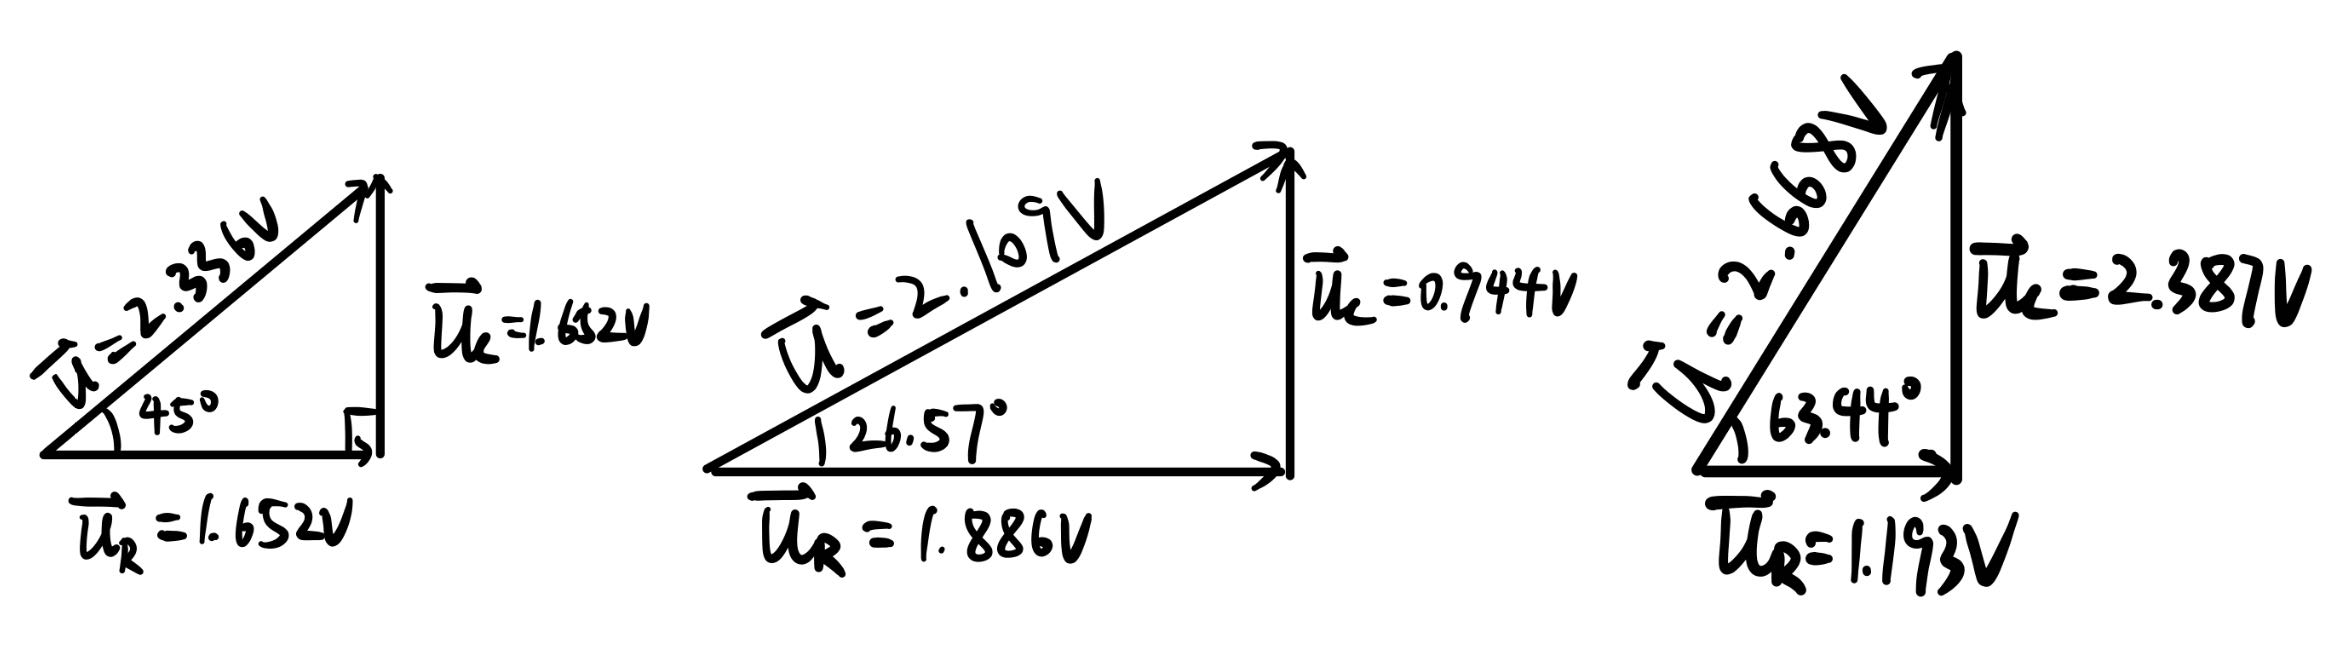
\includegraphics[width=0.8\textwidth]{graph3-1-1.jpg}
				\caption{RC电路电压三角形}
				\label{fig:graph3-1-1}
			\end{figure}

			可以发现$|U_R|^2+|U_C|^2\neq |U_0|^2= 9$,这是因为信号发生器自身存在内阻,在上次的实验中我们已经测定其内阻为$50\Omega$,加入这个修正后,$|U_R+U_{R_{eq}}|^2+|U_C|^2= |\frac{100+50}{100}\times U_R|^2+|U_C|^2\approx9$。如\cref{fig:graph3-1-2}

			\begin{figure}[htbp]
				\centering
				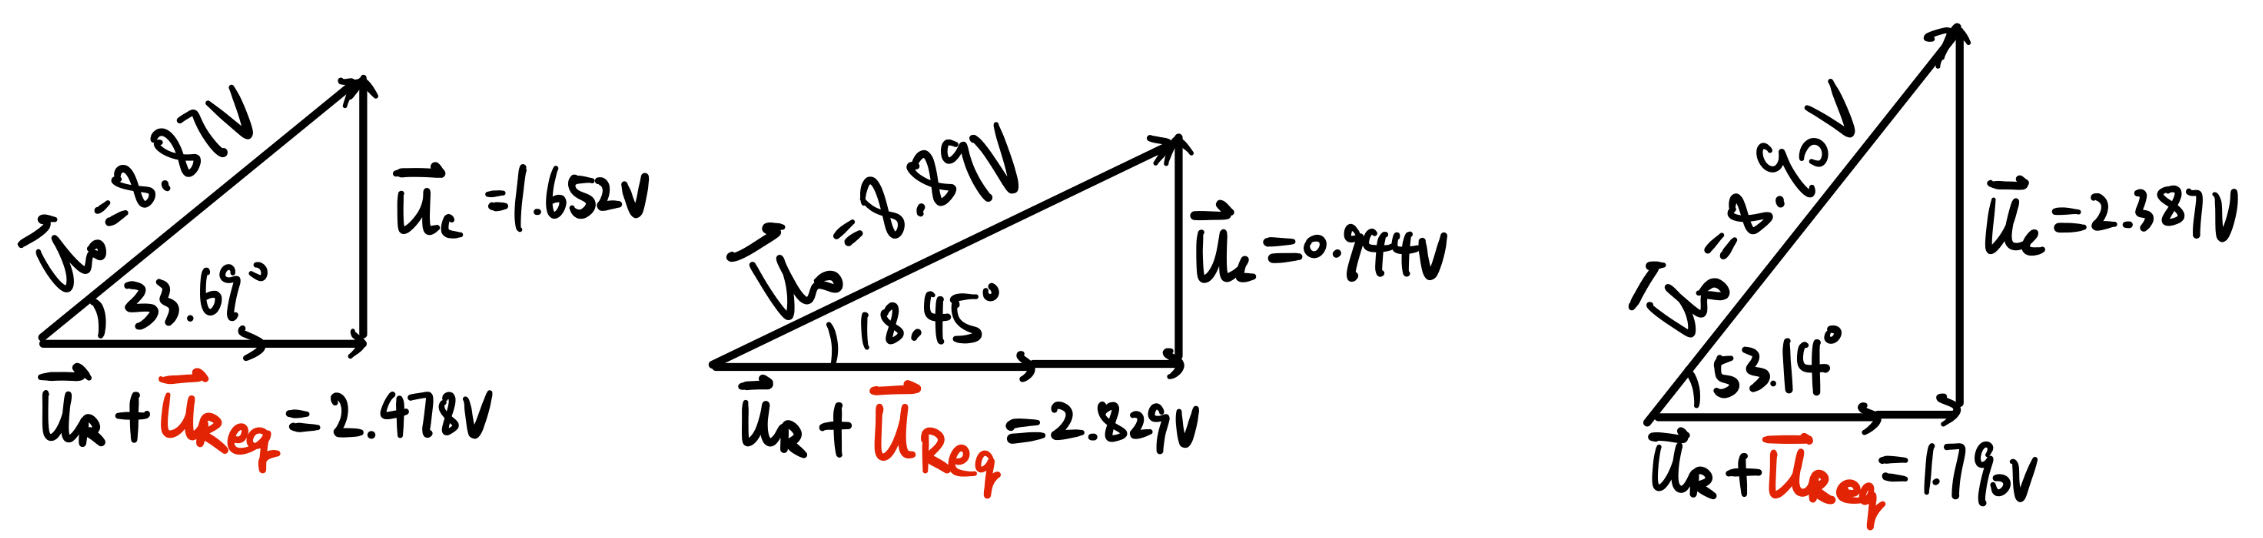
\includegraphics[width=0.8\textwidth]{graph3-1-2.jpg}
				\caption{\textbf{修正后}RC电路电压三角形}
				\label{fig:graph3-1-2}
			\end{figure}

			下面讨论RL电路的电压向量三角形:

			由\cref{tab-RL}可得到如下图像\cref{fig:graph3-1-3}

			\begin{figure}[htbp]
				\centering
				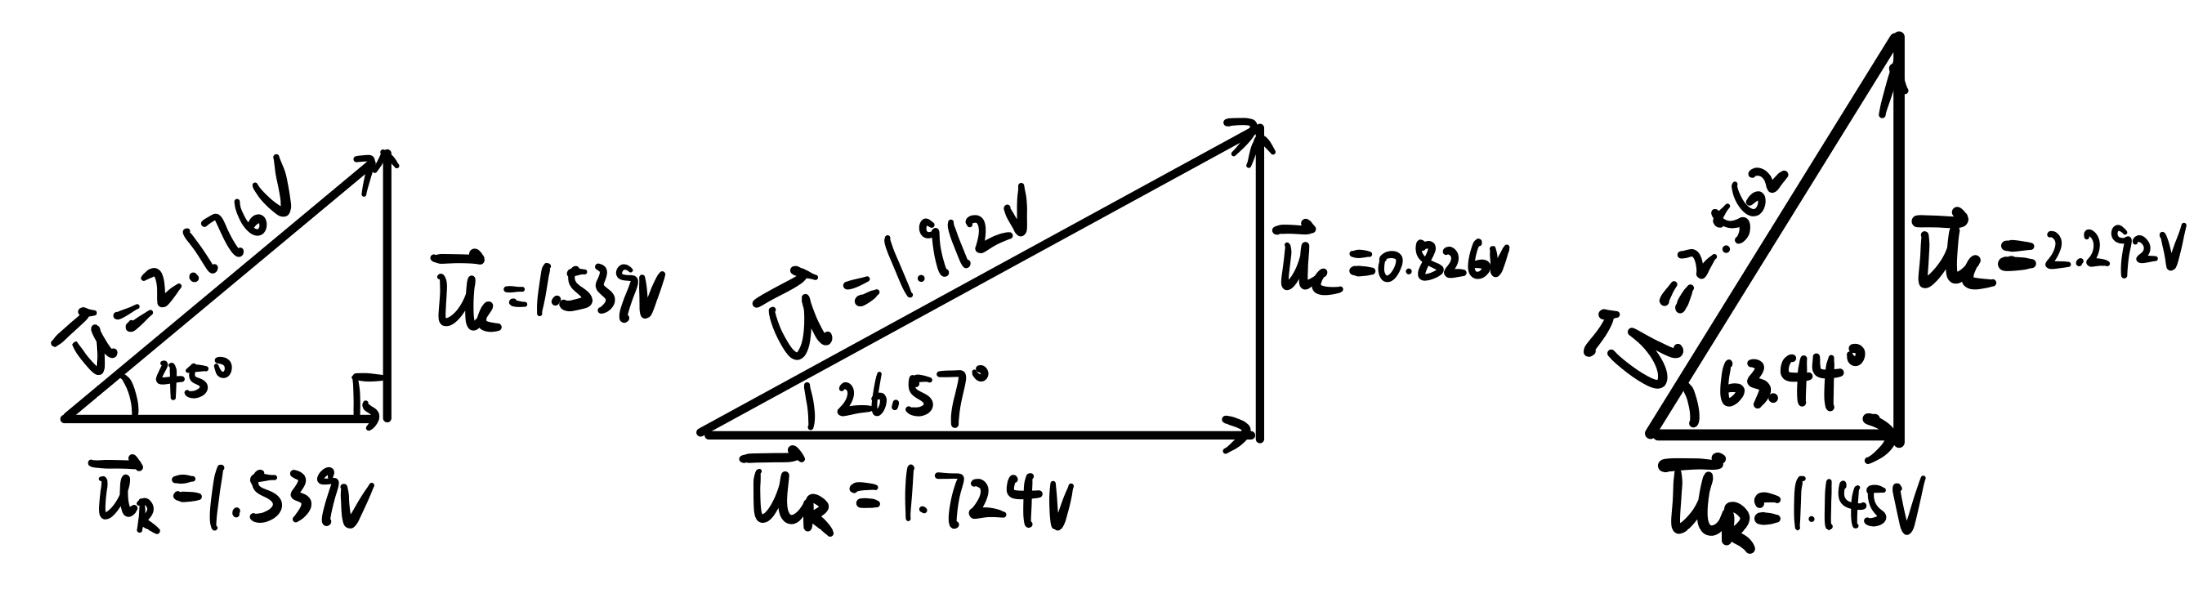
\includegraphics[width=0.8\textwidth]{graph3-1-3.jpg}
				\caption{RL电路电压三角形}
				\label{fig:graph3-1-3}
			\end{figure}

			可以发现$|U_R|^2+|U_C|^2\neq |U_0|^2= 9$,这是不仅是因为信号发生器自生存在内阻,电感自己也有一个内阻,由拟合结果知$R_L=9\Omega$,加入这个修正后,$|U_R+U_{R_{eq}}|^2+|U_C|^2= |\frac{100+50+9}{100}\times U_R|^2+|U_C|^2\approx9$。如\cref{fig:graph3-1-4}

			\begin{figure}[htbp]
				\centering
				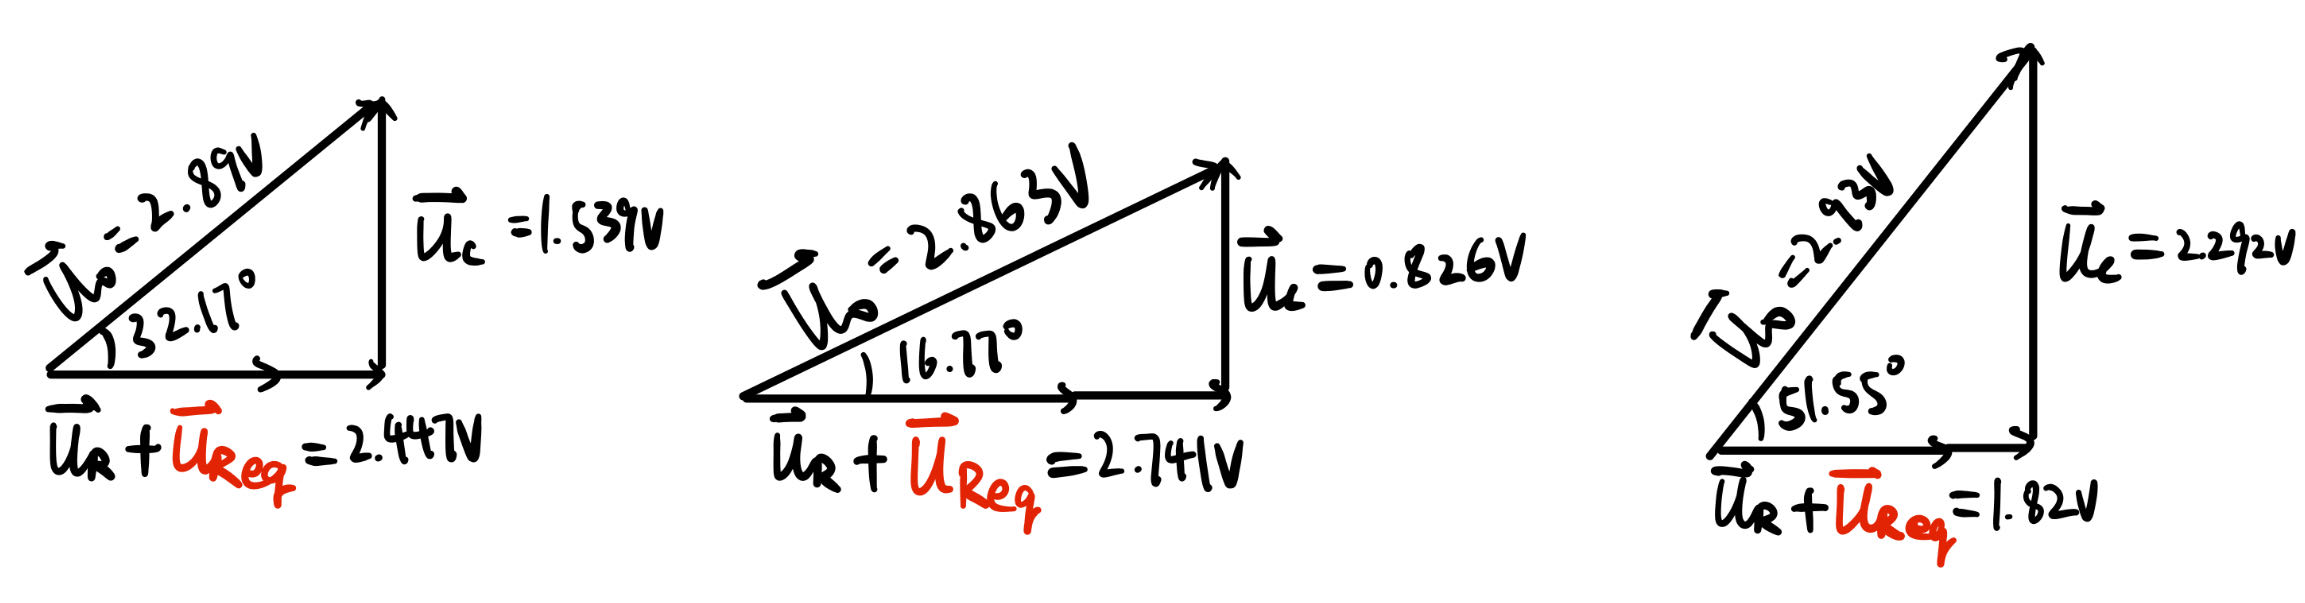
\includegraphics[width=0.8\textwidth]{graph3-1-4.jpg}
				\caption{\textbf{修正后}RL电路电压三角形}
				\label{fig:graph3-1-4}
			\end{figure}
			
		\item 阻抗三角形

			由实验数据\cref{{table:tbl-impedence}}绘制图像\cref{fig:ET1_6GraA3-1-3-4-1},\cref{fig:ET1_6GraA3-1-3-4-2}:

			\begin{figure}[htbp]
				\centering
				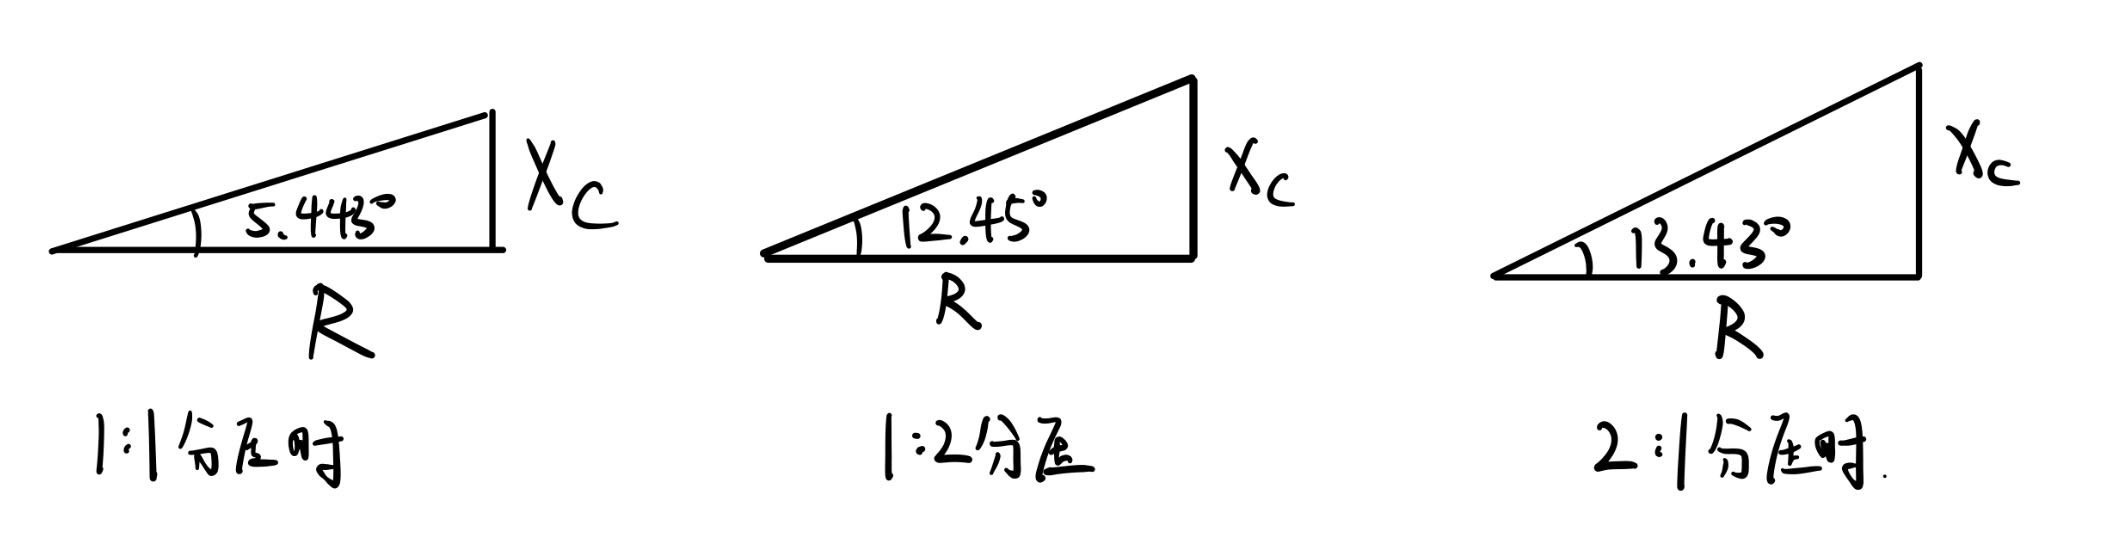
\includegraphics[width=0.8\textwidth]{ET1_6GraA3-1-3-4-1.jpg}
				\caption{\textbf{RC阻抗三角形}}
				\label{fig:ET1_6GraA3-1-3-4-1}
			\end{figure}

			\begin{figure}[htbp]
				\centering
				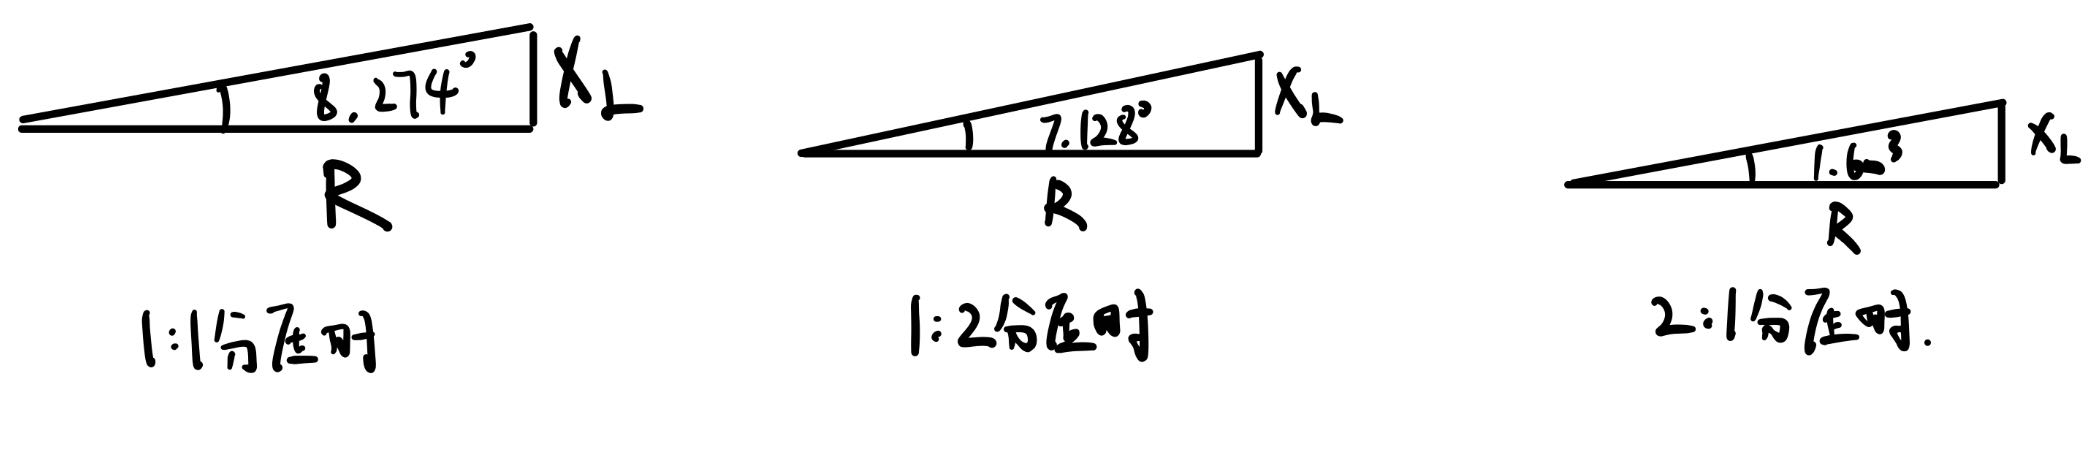
\includegraphics[width=0.8\textwidth]{ET1_6GraA3-1-3-4-2.jpg}
				\caption{\textbf{RL阻抗三角形}}
				\label{fig:ET1_6GraA3-1-3-4-2}
			\end{figure} 
			
			理论上电压三角形和阻抗三角形是相似的,但是实际测量发现差距较大。经过分析,可能是由于以下几个可能的误差来源导致的:

			\begin{enumerate}
				\item 测量误差:在使用双踪示波器测量相位差时,可能存在测量误差。示波器的相位测量功能可能受到信号波形的形状、噪声和示波器设置等因素的影响。这可能导致实际相位差的测量值偏离真实值。
		
				\item 连接误差:连接元件时,可能存在接触不良或连接不牢固的情况,导致信号波形的畸变或干扰,进而影响相位差的测量。
			
				\item 信号处理误差:在使用示波器测量信号时,信号处理电路可能会引入一定的延迟或失真,从而影响相位差的测量结果。
			
				\item 测量方法不准确:测量电压三角形和测量阻抗三角形所使用的方法可能存在差异或不够准确,导致最终测量结果不一致。
			\end{enumerate}

			% 为了减小这些误差,可以尝试以下方法:
		
			% \begin{enumerate}
			% 	\item 确保连接牢固,减小连接误差;
			% 	\item 校准示波器,确保其测量功能准确;
			% 	\item 使用不同的测量方法或设备,进行对比测量,以确定测量结果的准确性;
			% 	\item 多次重复实验,取平均值,以减小随机误差的影响。
			% \end{enumerate}
		
			
			
	\end{enumerate}
	
	%
	\subsubsection{幅频关系曲线}
	\begin{enumerate}
		\item 利用实验测得的数据(表)拟合幅频关系曲线
		
		\begin{figure}[htbp]
			\centering
			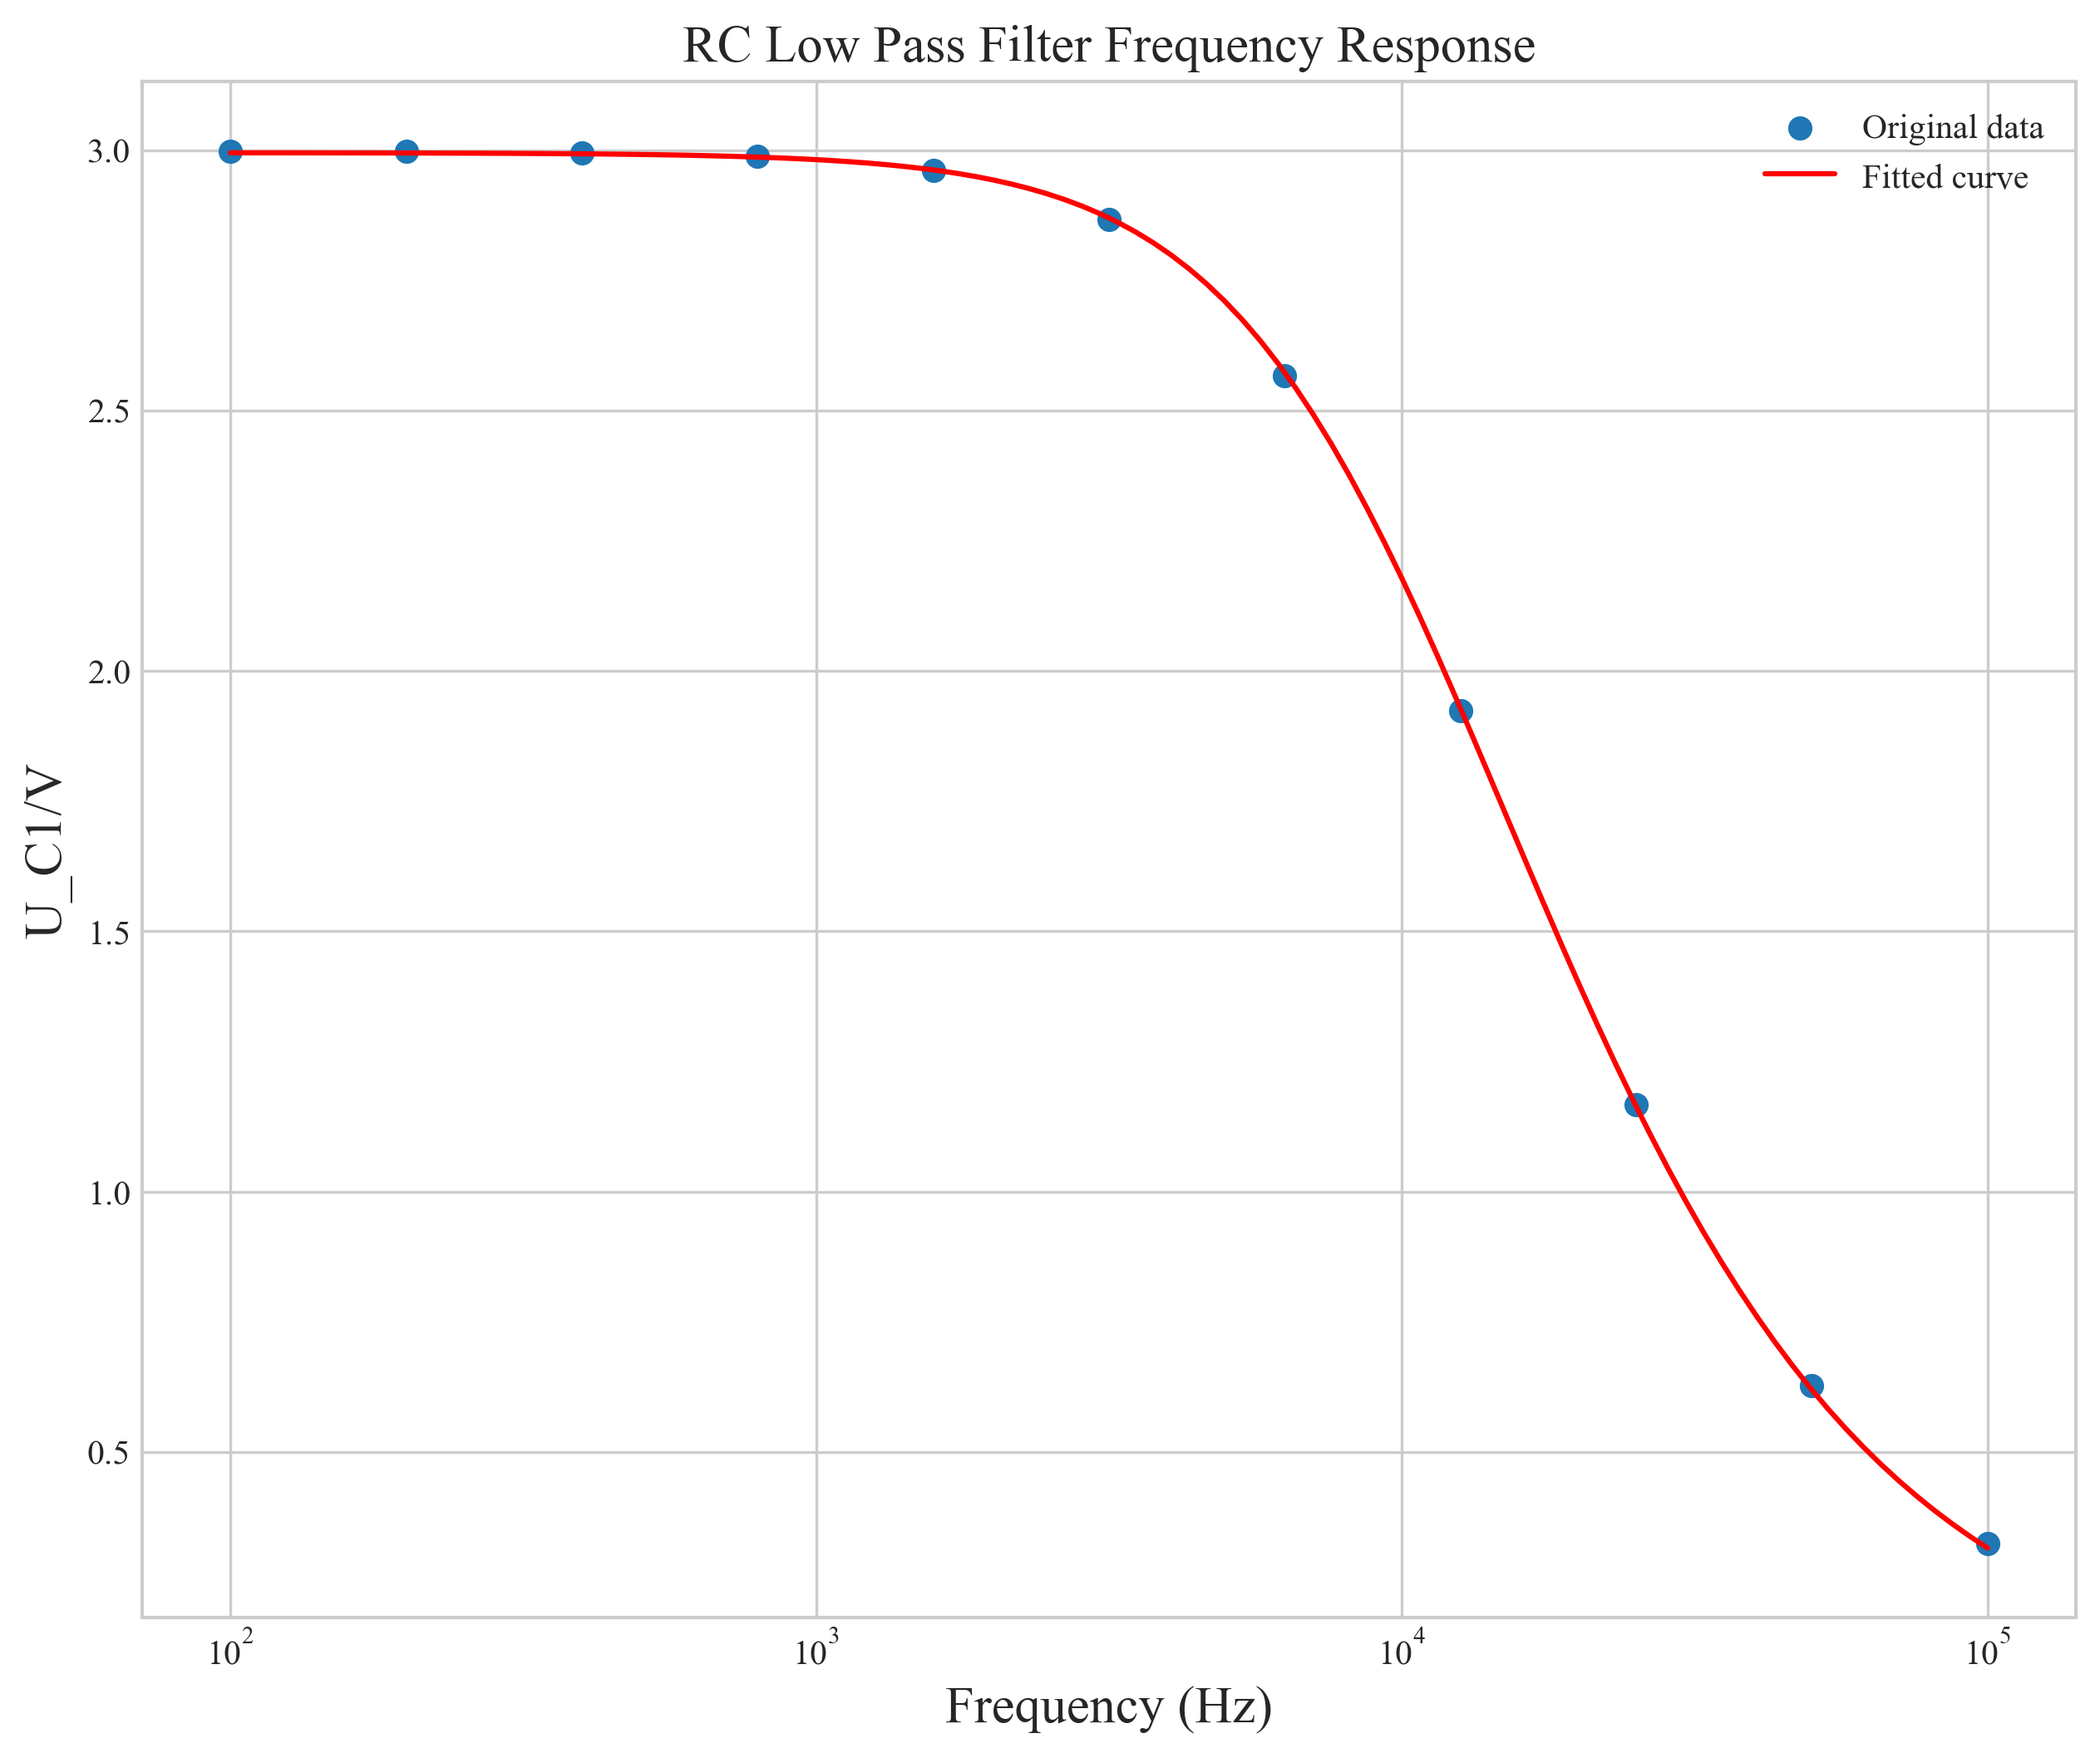
\includegraphics[width=0.5\textwidth]{ET1_6GraA1.png}
			\caption{C幅频关系曲线}
			\label{fig:figA1}
		\end{figure}
		
		\begin{figure}[htbp]
			\centering
			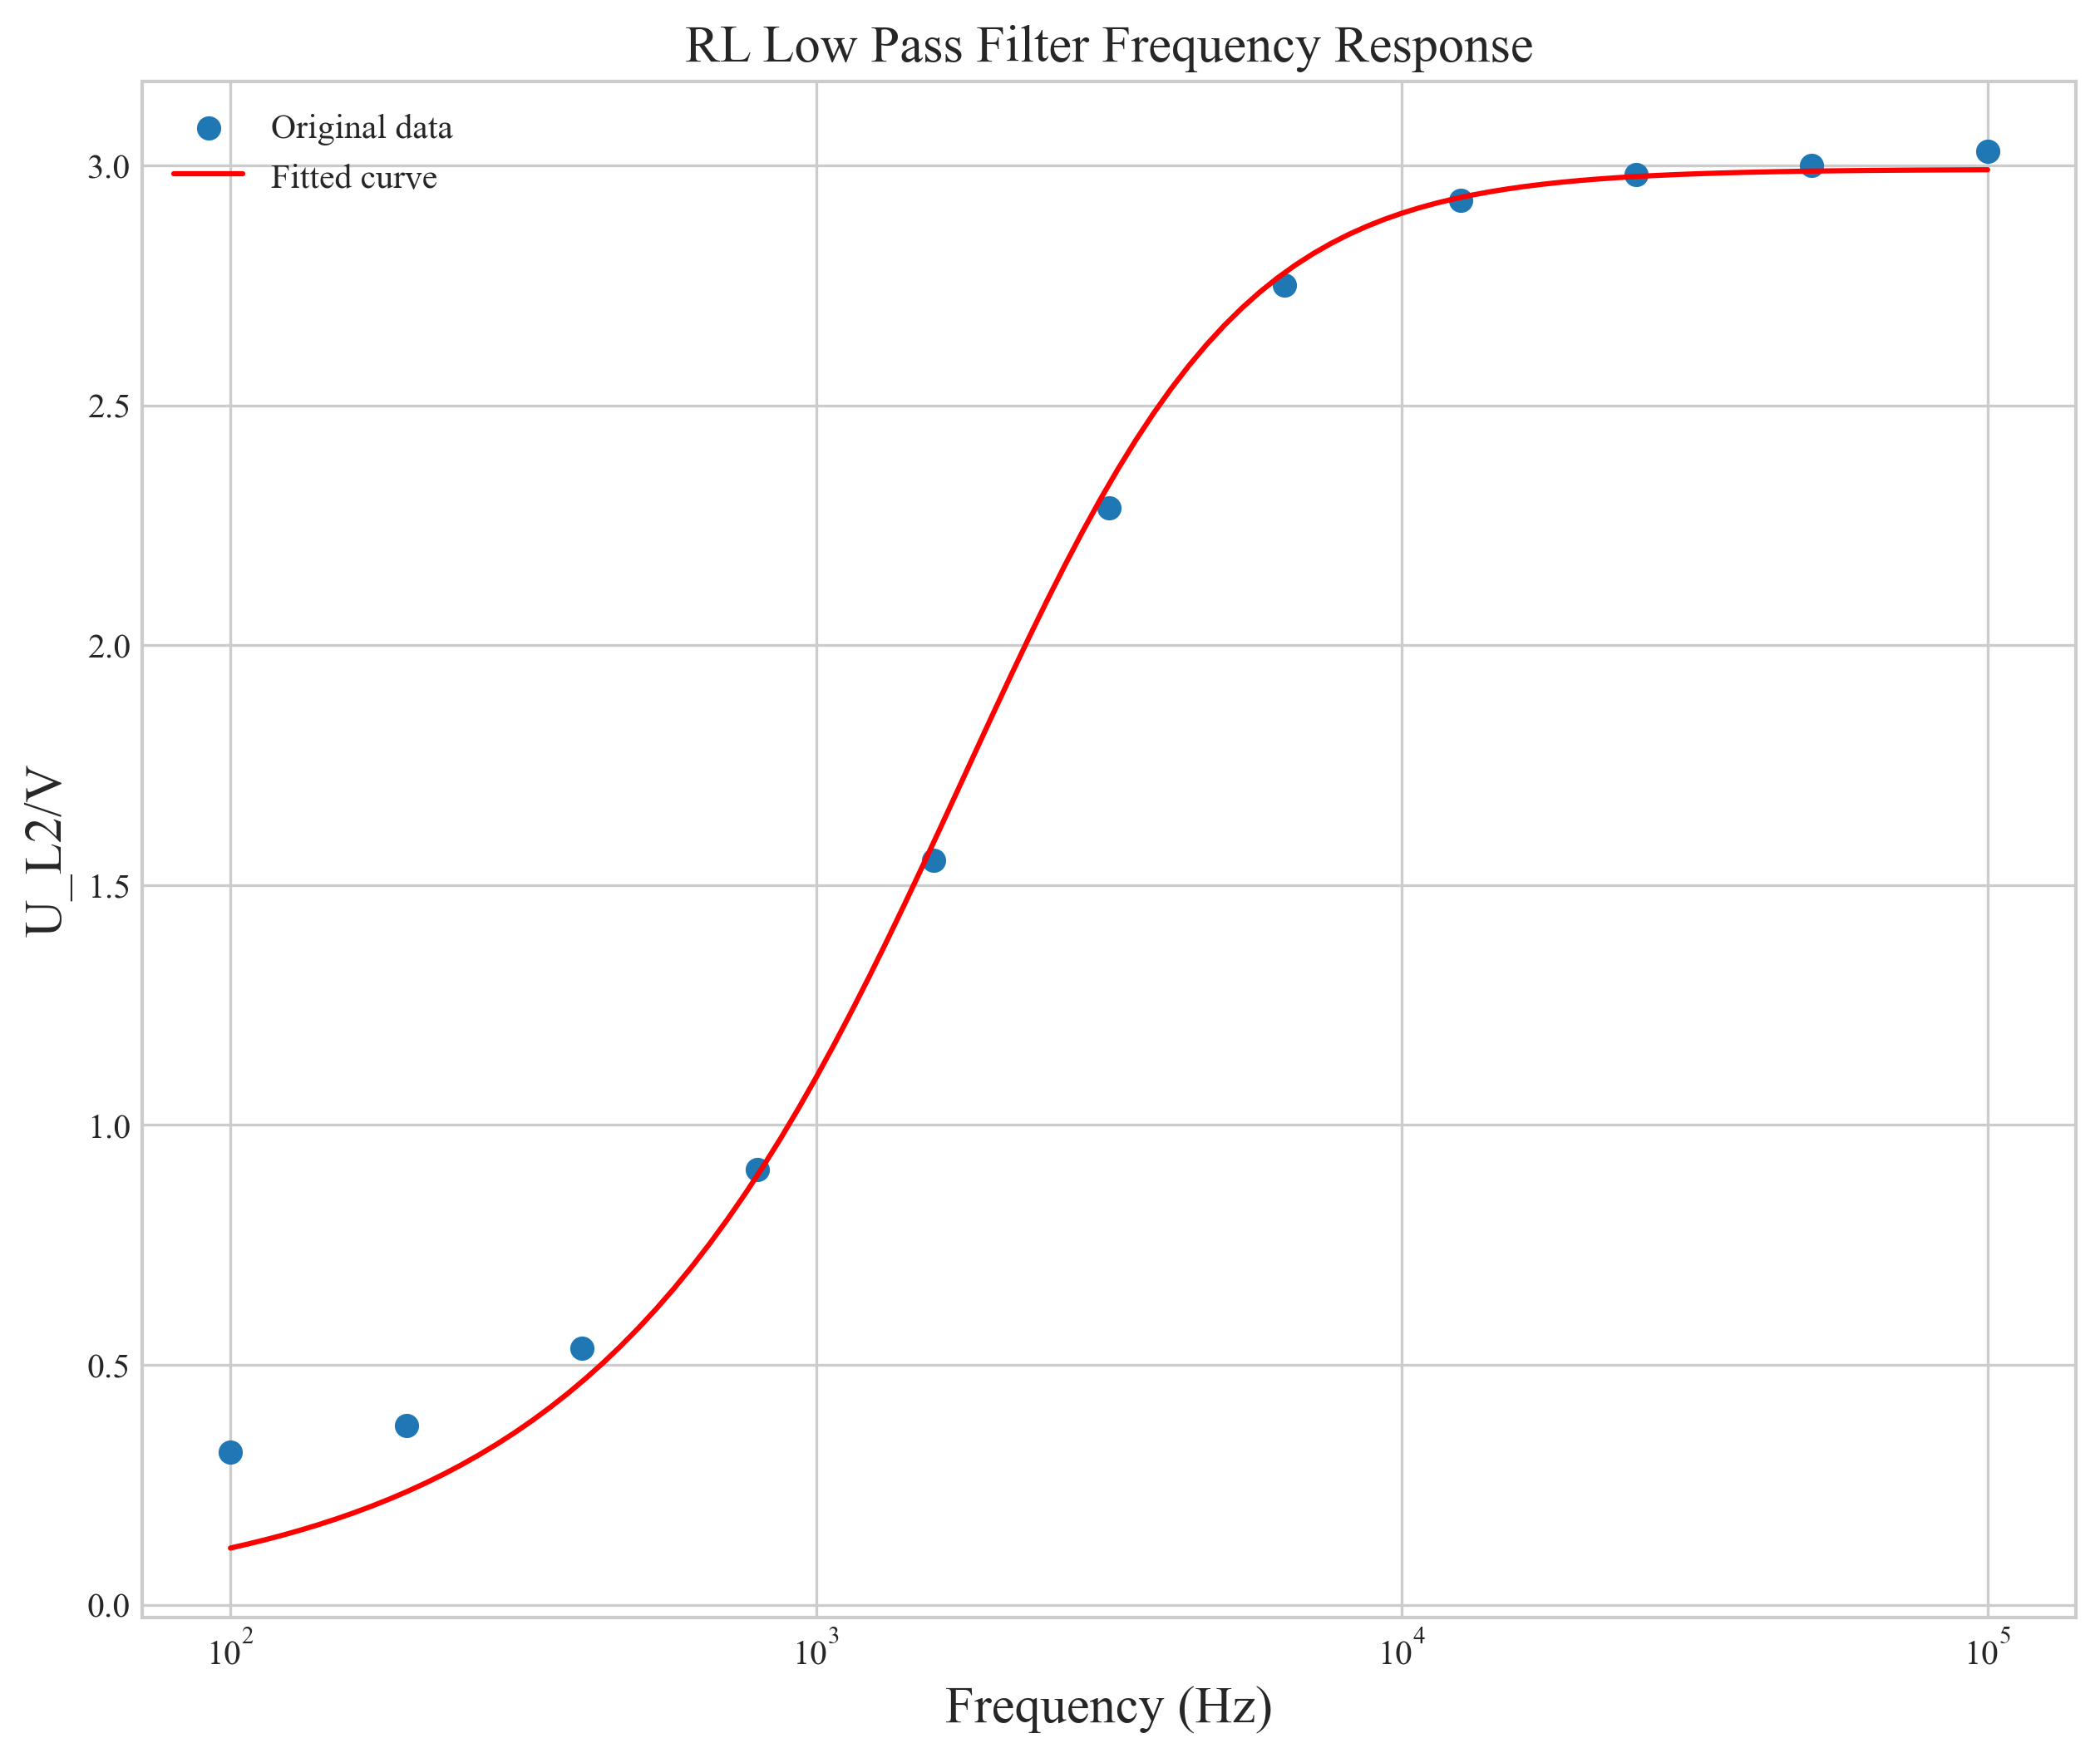
\includegraphics[width=0.5\textwidth]{ET1_6GraA2.png}
			\caption{L幅频关系曲线}
			\label{fig:figA2}
		\end{figure}
		
		\item 关于拟合参数的讨论
		
		从拟合参数我们可以计算出信号源内阻和电容、电感的自有总阻值,若引入已知的信号源内阻,则可以计算出相应的内阻值。
		
		拟合参数 (u, rc): [ 2.99488701e+00 -1.50285449e-05]	
		
		拟合参数 (u, r/l): [2.99220096e+00 1.59077822e+04]					
			
	\end{enumerate}
	
	%
	\subsubsection{相频关系曲线}
	\begin{enumerate}
		\item 利用实验测得的数据(表)绘制相频关系的样条曲线
		

			\begin{figure}[htbp]
				\centering
				\subfloat[电感的相频特性曲线实验数据图像]
				{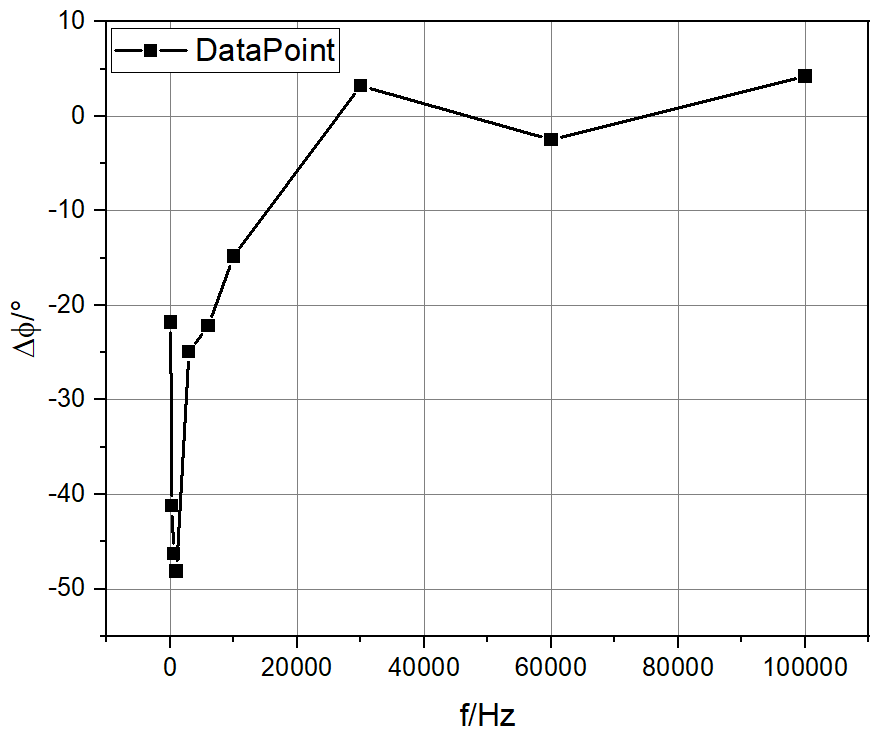
\includegraphics[width=0.4\textwidth]{graph3-1-3-3-4.png}\label{fig:graph3-1-3-3-4}}
				\quad
				\subfloat[电容的相频特性曲线实验数据图像]
				{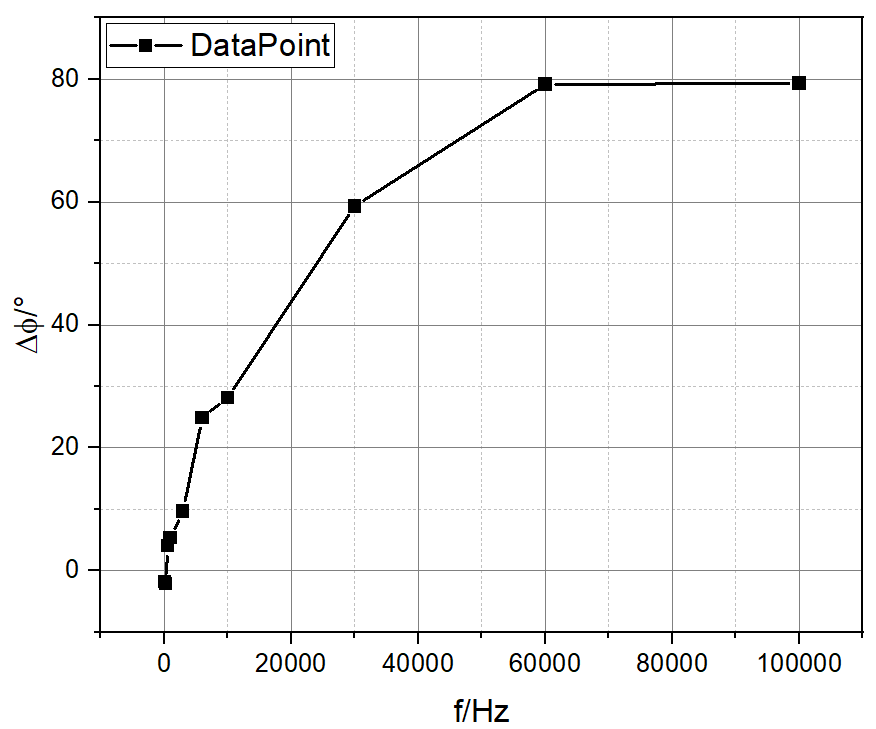
\includegraphics[width=0.4\textwidth]{graph3-1-3-3-3.png}\label{fig:graph3-1-3-3-3}}
				\quad
		
				\caption{实验数据绘制折线图}
				\label{fig:data}
			\end{figure}
		
		\item RC相频关系曲线拟合
		
		\begin{figure}[htbp]
			\centering
			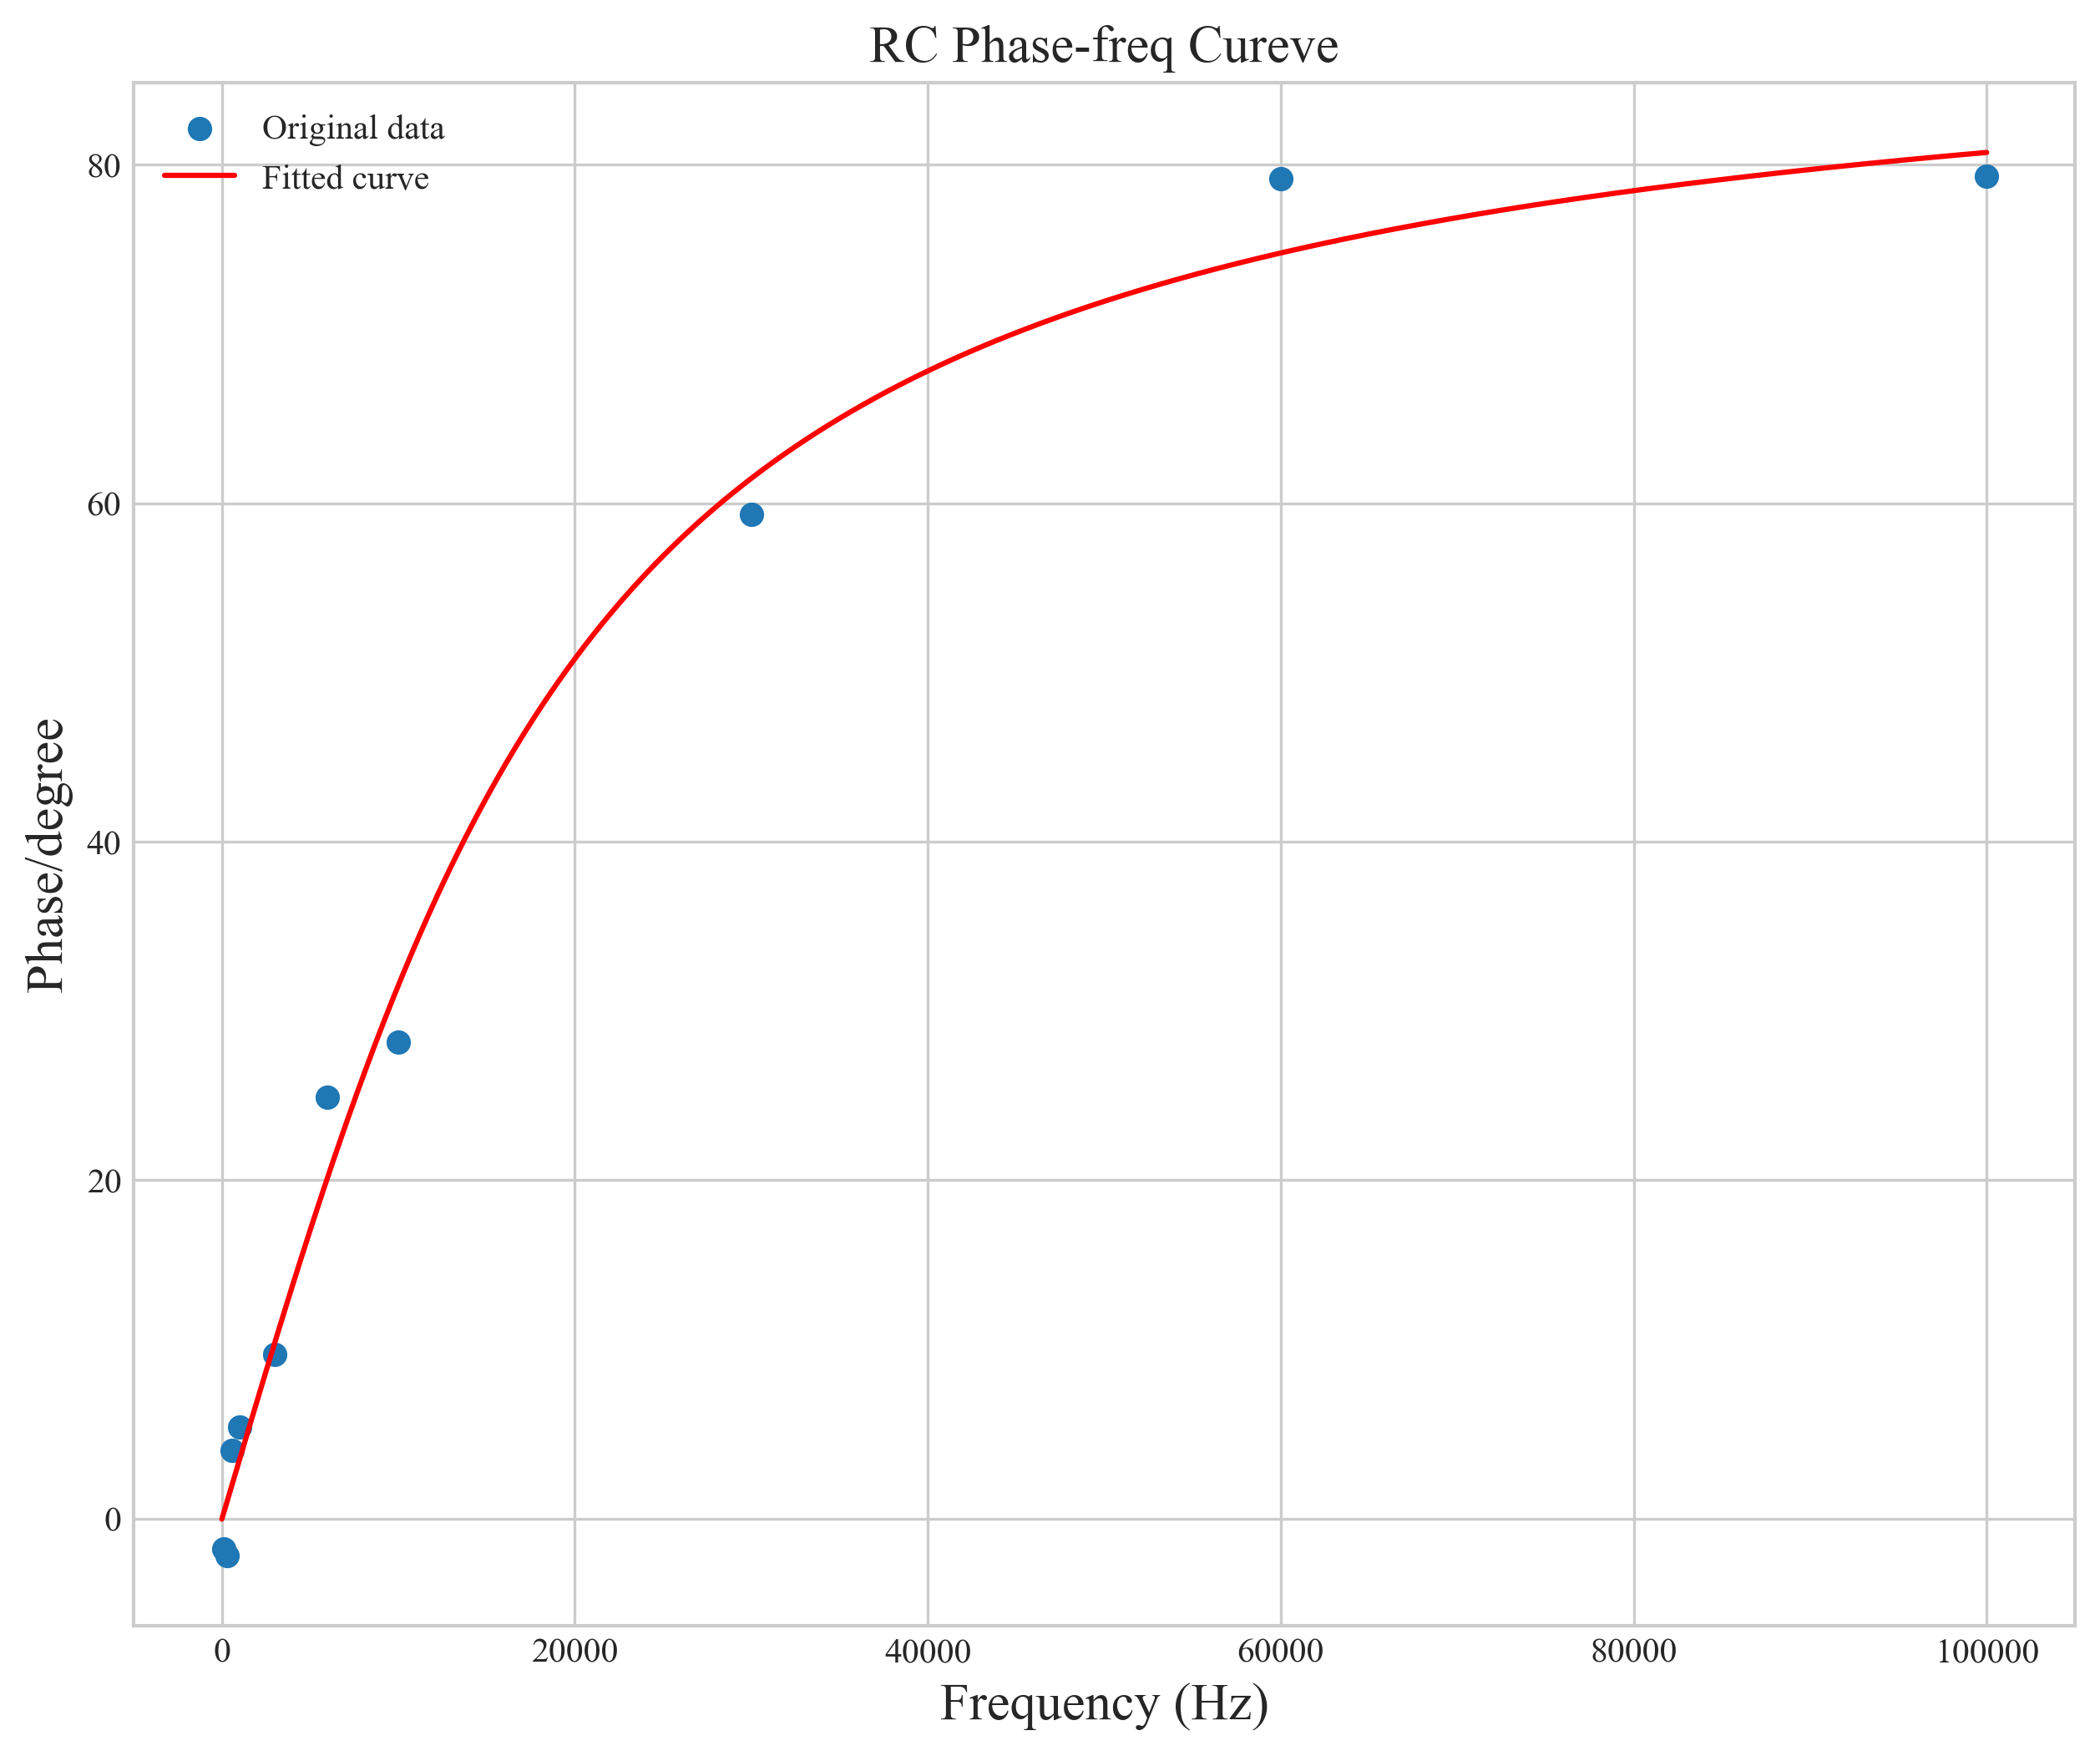
\includegraphics[width=0.5\textwidth]{ET1_6GraA3.png}
			\caption{RC相频关系曲线}
			\label{fig:figA3}
		\end{figure}
		
		\item 重新考虑RL与RC的模型并进行分析 

			\begin{enumerate}
				\item 实际电容的等效模型:
				
					理想的电容器在实际中是不存在的,电容的实际模型是一个电阻R串联一个电感L,再串联一个电容C,R是等效串联电阻,L是等效串联电感,C是理想的电容。

					\begin{figure}[htbp]
						\centering
						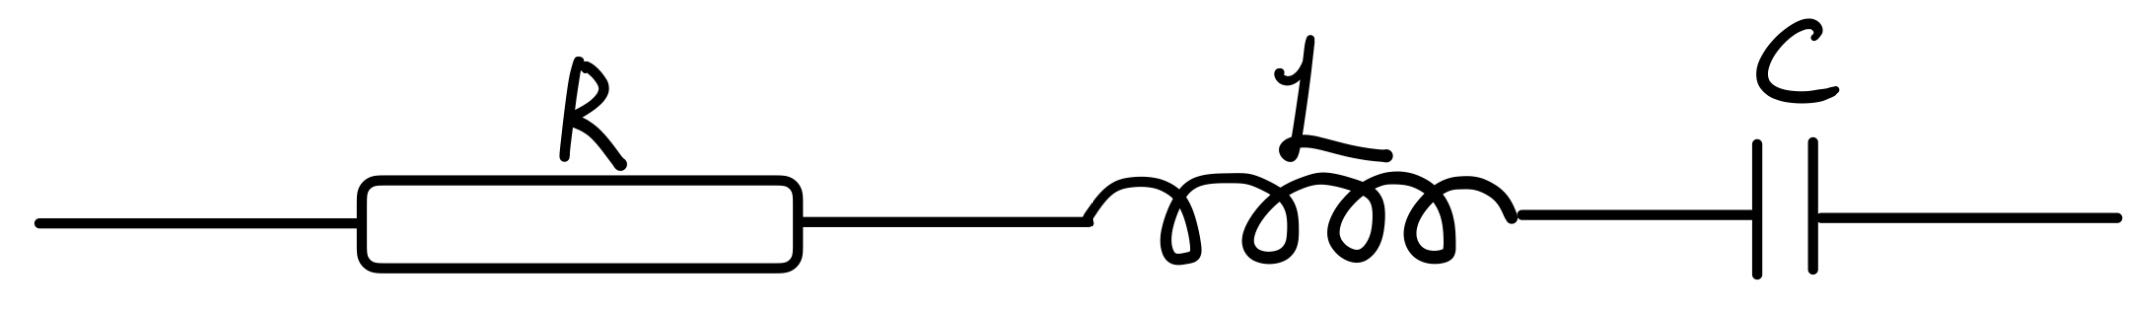
\includegraphics[width=0.4\textwidth]{graph3-1-3-3-1.jpg}
						\caption{实际电容的等效模型}
						\label{fig:graph3-1-3-3-1}
					\end{figure}

					则按照这个模型,电容的阻抗应为:$Z=R+j\omega L+\frac{1}{j\omega C}=R+j(\omega L-\frac{1}{\omega C})$

					\begin{enumerate}
						\item 在$\omega L\ll \frac{1}{\omega C}$时,电容器表现为容性;
						\item 在$\omega L\gg \frac{1}{\omega C}$时,电容器表现为感性;
						\item 在$\omega L =  \frac{1}{\omega C}$时,此时容抗矢量等于感抗矢量,电容的总阻抗最小,表现为纯电阻特性,此时的f称为电容的自谐振频率。
					\end{enumerate}



					从\cref{fig:graph3-1-3-3-3}可以看到阻抗角随着频率的增加而增加,并没有极值出现.这说明其寄生电感$L$很小,其感性基本无法体现出来.则该电容器很接近理想电容器.

					% 自谐振频率点是区分电容是容性还是感性的分界点,高于谐振点时,“电容不再是电容”,因此退耦作用将下降。实际电容器都有一定的工作频率范围,在工作频率范围内,电容才具有很好的退耦作用。$L$是电容在高于自谐振频率点之后退耦功能被消弱的根本原因。


				\item 实际电感的等效模型:
				
					理想的电感在实际中也是不存在的,其实际模型应当是一个电阻R串联一个电感L,在并联一个电容C,R是等效串联电阻,L是等效串联电感,C是理想的电容。

					按照这个模型,电感的阻抗应为:$Z=\frac{(j\omega L+R)\times\frac{1}{j\omega C}}{j\omega L+R+\frac{1}{j\omega C}}=\frac{j\omega L+R}{(1-\omega^2LC)+j\omega RC}$

					\begin{figure}[htbp]
						\centering
						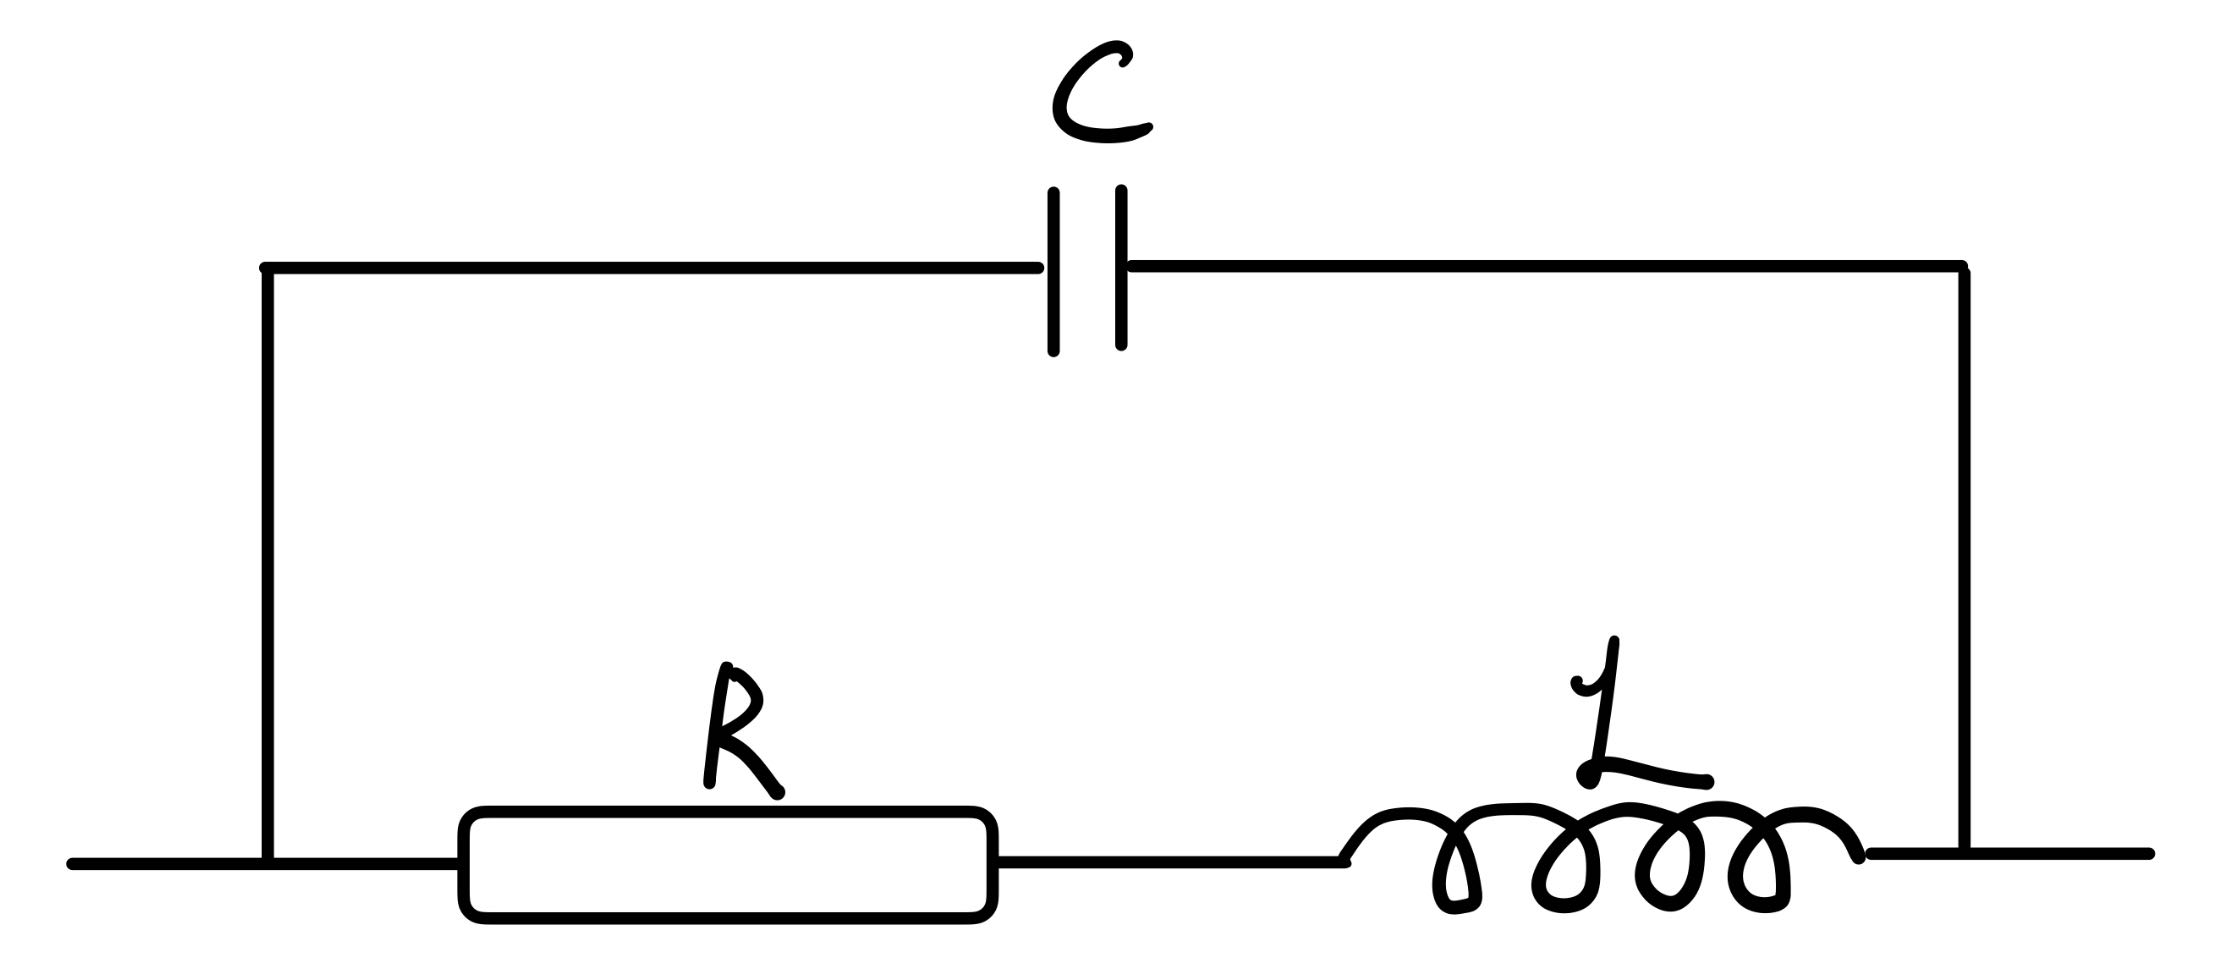
\includegraphics[width=0.4\textwidth]{graph3-1-3-3-2.jpg}
						\caption{实际电感的等效模型}
						\label{fig:graph3-1-3-3-2}
					\end{figure}

					\begin{enumerate}
						\item 在$\omega L\ll \frac{1}{\omega C}$时,电感表现为感性;
						\item 在$\omega L\gg \frac{1}{\omega C}$时,电感表现为容性;
						\item 在$\omega L =  \frac{1}{\omega C}$时,容抗和感抗相互抵消,电感呈现纯阻性,此时电感的阻抗最大
					\end{enumerate}

					由\cref{fig:graph3-1-3-3-4}可以看到,该电感在高频时,随着频率增加.阻抗角逐渐减小至0,仍然表现出电感的特性,说明其寄生电容很小,在100KHz时也不会体现出电容的特性。

					但是在低频时,数据明显发生了偏离理想电感的情况,可能的原因有:
						\begin{enumerate}
							\item 自谐振效应:电感器在低频时可能会出现自谐振现象。自谐振是指电感器的电感和寄生电容之间的共振,导致阻抗变化。这会影响电感器的性能,使其在低频下表现不佳。
							\item 线圈寄生效应:实际电感器中存在线圈寄生效应,如分布电容和铁芯/铜线电阻损耗。这些效应会随着频率变化而发生显著的变化,影响电感器的阻抗特性。
							\item 测试仪表误差:测试仪表在不同频率下的精度可能不同。低频信号的测量可能受到仪表误差的影响,导致测量结果不够准确。
							\item 电路寄生效应:电路中其他元件和布线也会影响电感器的频率响应。例如,布线的电阻和电容会与电感器产生耦合,影响其性能。
						\end{enumerate}


					



					% 由实验数据图像可发现,阻抗角有一个明显的极值:从$f=100Hz$开始,阻抗角的绝对值逐渐增大,到达一个极值后,阻抗角的绝对值逐渐减小至0.这符合我们所考虑的等效模型.说明其等效电容$C$是不能被忽略的.



			\end{enumerate}
			
	\end{enumerate}
	
	
	% ---
	
	% 实验后思考题
	%\subsection{实验后思考题}
	
	% ---
	
	
	% 结语部分
	\clearpage
	
	% 小标题
	\section{ET1-6 R、L、C元件阻抗特性研究 \quad\heiti 结语}
	% ---
	
	% 总结、杂谈与致谢
	%\subsection{实验心得和体会、意见建议等}
	
	% ---
	
	% 参考文献
	\subsection{参考文献}
	[1] 维基百科 https://zh.wikipedia.org
	
	[2] 电子技术实验 保延翔 2020.07 中山大学公共实验教学中心
	
	% ---
	
	% 附件
	\subsection{附件及实验相关的软硬件资料等}
	%试验台桌面整理如%\cref{}所示。
	
	实验报告个人签名如\cref{fig:name}。
	
	\begin{figure}[htbp]
		\centering
		\subfloat[]{
			
\includegraphics[width=0.45\textwidth]{name.png}
		}
		\subfloat[]{
			
\includegraphics[width=0.45\textwidth]{name-TaLEs.jpg}
		}
		\caption{个人签名}
		\label{fig:name}			
	\end{figure}
	
	% ---
	
	相关代码已上传至Github。
	
	
	
\end{document}